\documentclass[11pt]{article}
% Keep release builds byte-stable by omitting volatile engine timestamps and IDs.
\ifdefined\pdfinfoomitdate\pdfinfoomitdate=1\fi
\ifdefined\pdftrailerid\pdftrailerid{}\fi
\ifdefined\pdfsuppressptexinfo\pdfsuppressptexinfo=-1\fi
\usepackage[T1]{fontenc}
\usepackage[utf8]{inputenc}
\usepackage{lmodern}
\usepackage[margin=1in]{geometry}
\usepackage{amsmath,amssymb,amsthm,mathtools}
\usepackage{booktabs,array,microtype}
\usepackage{graphicx}
\usepackage{needspace}
\usepackage[round,authoryear]{natbib}
\usepackage[colorlinks=true,linkcolor=blue,citecolor=blue,urlcolor=blue]{hyperref}
\hypersetup{
pdftitle={Quoting Under a Misspecified Fill Law},
pdfauthor={Miquel Noguer Alonso},
pdfsubject={Order-book queues, adverse selection, and inventory-control certificates. DOI: 10.5281/zenodo.22759528},
pdfkeywords={market making, order-book queues, adverse selection, inventory control, model misspecification}}
\setlength{\emergencystretch}{3em}
\theoremstyle{plain}
\newtheorem{theorem}{Theorem}[section]
\newtheorem{proposition}[theorem]{Proposition}
\newtheorem{corollary}[theorem]{Corollary}
\newtheorem{lemma}[theorem]{Lemma}
\theoremstyle{definition}
\newtheorem{definition}[theorem]{Definition}
\newtheorem{assumption}[theorem]{Assumption}
\newtheorem{example}[theorem]{Example}
\theoremstyle{remark}
\newtheorem{remark}[theorem]{Remark}
\newcommand{\E}{\mathbb E}
\newcommand{\R}{\mathbb R}
\newcommand{\dd}{\,\mathrm d}
\newcommand{\norm}[1]{\lVert#1\rVert}
\newcommand{\HH}{\mathcal H}
\newcommand{\cAct}{\mathcal A}
\newcommand{\XX}{\mathcal X}
\DeclareMathOperator{\TV}{TV}
\DeclareMathOperator{\KL}{KL}
\DeclareMathOperator{\spn}{span}
\DeclareMathOperator{\dist}{dist}

\title{Quoting Under a Misspecified Fill Law:\\
Order-Book Queues, Adverse Selection,\\
and Inventory-Control Certificates}
\author{Miquel Noguer Alonso\\
\small Artificial Intelligence Finance Institute}
\date{15 September 2026\\[5pt]\small DOI:
\href{https://doi.org/10.5281/zenodo.22759528}{10.5281/zenodo.22759528}}
\begin{document}
\maketitle
\begin{abstract}
A market maker's fill law depends on price, tagged queue priority,
order size, order flow, and price changes accompanying execution.
This paper connects uncertainty in these book primitives to the
loss of a deployed quoting policy. A marked-wealth identity separates
offset capture, carried-inventory drift, and simultaneous fill--price
jumps. A finite event model retains inventory reservations, batch
consumption, partial fills, and costly replacement. A pending
cancellation remains executable until acknowledgement. Its value
admits an exact residual identity and a perturbation bound in the
delay law. Approximating a deterministic delay by mean-matched
Erlang stages has a sharp inverse-stage value-error rate, with an
explicit leading term and remainder.
A performance-difference identity transfers local decision errors
into total policy loss. Smooth quote branches admit quadratic
certificates accounting for primitive uncertainty, continuation
values, HJB residuals, and optimization error. Discrete messages
admit a value-interval certificate that preserves state-dependent
action gaps and bounds their discounted occupation. It requires
neither action curvature nor the true value function. A 74-state
queue-and-inventory example gives a rational loss enclosure for
a declared uncertainty box. Two lower bounds identify limits:
omitting tagged rank causes positive minimax loss with known
primitives, while calibration at a replacement boundary has a sharp
inverse-square-root duration rate. A separate two-quote experiment
gives a statistical certificate for an exponential fill curve.
Hybrid margins, finite-book truncation, shutdown thresholds,
and information-value ceilings receive explicit assumptions.
The guarantees are conditional on specified models and uncertainty
sets. Synthetic examples independently check partial-fill laws,
cancellation values, controlled policies, and the resulting bounds.
\end{abstract}
\noindent\textbf{Keywords:} market making; adverse selection; marked point
processes; queue priority; inventory control; model misspecification.

\clearpage
\tableofcontents
\clearpage

\section{Introduction}

Market making combines a quoting decision with an inventory decision.
A quote determines which counterparties trade, the inventory they leave,
and the information their trades reveal. These effects make the fill law
more than a demand curve: it is also part of the controlled transition
law and the distribution of post-fill price changes.

Inventory models descend from \citet{HoStoll1981}, and adverse-selection
models from \citet{GlostenMilgrom1985}. The quoting frameworks of
\citet{AvellanedaStoikov2008}, \citet{GueantLehalleFernandezTapia2013},
and \citet{CarteaJaimungalPenalva2015} explain how execution probabilities
interact with inventory costs. Model uncertainty in arrival rates, fill
probabilities, and price dynamics is explicitly studied by
\citet{CarteaDonnellyJaimungal2017}. Thus neither uncertain fills nor
inventory-sensitive quotes are new modeling ingredients.
More directly, \citet{CaoEtAl2026} obtain a second-order performance gap
and a logarithmic-squared learning-regret bound for an ergodic
Avellaneda--Stoikov model. Quadratic sensitivity of a market-making
policy is therefore also an established phenomenon.

The question developed here is a quantitative transfer question:
given a policy optimized under one fill-and-price law, what bounds its
performance under another? A one-step quote certificate is insufficient
for this purpose. The estimated law changes the inventory shadow price
as well as the immediate reward, and the policy visits states according
to the true controlled dynamics.

Section~\ref{sec:bookevents} makes the book interpretation explicit.
It distinguishes a displayed queue from the position of a tagged order,
retains live orders during pending cancellation, and models replacement
as a state reset. Proposition~\ref{prop:eventbudgets} maps errors in
event rates and conditional price marks to the primitive budgets used
by the control certificates. Proposition~\ref{prop:booktruncation}
adds a separate allowance for exiting a finite retained cell. Queue
absorption methods themselves are established
\citep{ContStoikovTalreja2010}; their role here is to identify which
execution law, state variables, and approximation errors the
misspecification comparison must retain.
Section~\ref{sec:partialfills} extends this construction to
batch consumption and partial fills, preserving the association
between executed volume and its price mark.
Theorems~\ref{thm:cancellationvalue} and \ref{thm:erlanglatency}
then retain fills during pending cancellation and quantify the
value error of a finite-stage delay model. The latter gives a
mean-matched expansion with a sharp \(k^{-1}\) leading order,
rather than identifying small timing variance with negligible
economic loss.

Theorem~\ref{thm:dynamiccertificate} addresses this
distinction. It combines a finite-state performance-difference identity
with a constrained strong-concavity estimate. Corollary~\ref{cor:primitive}
then bounds the gradient discrepancy using errors in primitive rewards
and transition rates, including the resulting error in continuation
values. Theorem~\ref{thm:computable} extends this comparison to a numerically
computed value function and an inexact optimizer. It uses supplied
primitive uncertainty bounds, an HJB residual, a terminal discrepancy,
and a verified curvature enclosure; its right side does not require
the true value function. Theorem~\ref{thm:hybrid} adds a separate
occupation-margin term for hybrid actions. Proposition~\ref{prop:coverage}
shows why arbitrarily much data at one quote cannot by itself justify
vanishing uncertainty away from that quote. Proposition~\ref{prop:twoquote}
provides the positive counterpart under a two-quote Poisson experiment.
Theorem~\ref{thm:discounted} gives the stationary discounted extension,
and Corollary~\ref{cor:discountedcomputed} retains numerical errors in that
setting. For discrete quote messages, Theorem~\ref{thm:intervalcontrol}
encloses model-specific values and then evaluates a state-dependent
upper bound on the deployed policy's action gaps. This avoids
discarding the queue states in which an error can occur.
Section~\ref{sec:intervalexample} implements that comparison with
rational arithmetic in a continuing 74-state inventory model.
Proposition~\ref{prop:ranklower} and
Theorem~\ref{thm:queuestatrate} give complementary lower bounds:
one for omitted tagged rank and one for finite calibration near
a replacement boundary.

The finite-horizon and discounted certificates concern marked
rewards and general controlled rates. The two-quote experiment measures
post-calibration revenue loss; it does not supply an online learning
algorithm or improve the ergodic learning rate of \citet{CaoEtAl2026}.

Three distinctions organize the analysis. Carried-inventory drift and
fill--price co-jumps are separate accounting terms. A local quote
Hamiltonian and a total policy objective are separate optimization
objects. Finally, a smooth quote adjustment and a discrete decision to
withdraw a quote have different stability requirements.

The execution monograph \citep{NoguerAlonso2026Execution} studies a
parent mandate, its conserved ledger, and error certificates for feasible
execution policies. This paper concerns continuing liquidity provision:
there is no prescribed quantity to complete, and inventory is a state
whose cost enters the objective. The common object is a feasible policy
evaluated under a specified information class. Here the accounting
needed for that comparison includes simultaneous fills and price jumps,
and the stability calculation separates smooth offsets from discrete
participation decisions.

\section{Wealth accounting with simultaneous fills and price jumps}

Fix a finite horizon \(T\) and a filtered probability space satisfying the
usual conditions. The reference price is a special semimartingale
\[
S_t=S_0+M_t+A_t,\qquad M_0=A_0=0,
\]
where \(M\) is a local martingale and \(A\) is predictable with finite
variation. Unit ask and bid fills are counted by \(N^a,N^b\), with
predictable intensities \(\Lambda^a_t,\Lambda^b_t\).
Predictable offsets \(\delta^a_t,\delta^b_t\ge0\) generate cash and inventory
\[
\dd K_t=(S_{t-}+\delta^a_t)\dd N^a_t
        -(S_{t-}-\delta^b_t)\dd N^b_t,\qquad
q_t=q_0+N^b_t-N^a_t.
\]
Wealth is \(W_t=K_t+q_tS_t\). Quotes are priced relative to the pre-jump
reference \(S_{t-}\).

\begin{assumption}[Integrable admissible policies]\label{ass:accounting}
Offsets and intensities are bounded, \(q\) is bounded, and
\[
\E[M]_T<\infty,\qquad
\E\operatorname{Var}_{[0,T]}(A)<\infty.
\]
Counting processes are nonexplosive, have unit jumps, and have no common
ask--bid jumps. An inactive side has intensity zero; monotonicity of
intensity in its offset is required only on an active side when used
later. Inventory constraints are enforced through admissible order
states: a side whose execution would violate the bound must already
be inactive.
\end{assumption}

The last convention permits a bounded-inventory model. It cannot be
implemented by suppressing the execution of an order that remains live.
The reservation invariant in Section~\ref{sec:bookevents} gives an
explicit admissible-state construction, including pending messages.

\begin{theorem}[Three-term wealth decomposition]\label{thm:accounting}
Under Assumption~\ref{ass:accounting},
\begin{align}
\E[W_T-W_0]
={}&\E\int_0^T(\delta^a_t\Lambda^a_t+\delta^b_t\Lambda^b_t)\dd t
 +\E\int_0^Tq_{t-}\dd A_t \notag\\
&+\E\sum_{0<t\le T}\Delta q_t\,\Delta S_t .\label{eq:wealth}
\end{align}
All terms in this equality are finite.
\end{theorem}
\begin{proof}
Integration by parts gives
\[
\dd W_t=\delta^a_t\dd N^a_t+\delta^b_t\dd N^b_t
       +q_{t-}\dd S_t+\dd[q,S]_t.
\]
The process \(q\) has finite variation and is purely discontinuous, hence
\([q,S]_T=\sum\Delta q_t\Delta S_t\).
Bounded predictable integrands and \(\E[M]_T<\infty\) make
\(\int q_-\dd M\) a square-integrable martingale. Its expectation is zero.
The counting-process integrals have the stated compensators.

To check absolute integrability of the bracket, put \(N=N^a+N^b\).
Then \(|\Delta q|\le1\) and
\[
\sum_{t\le T}|\Delta q_t\Delta M_t|
\le \sqrt{N_T}\sqrt{[M]_T}.
\]
Its expectation is finite by Cauchy--Schwarz, since bounded intensities
give \(\E N_T<\infty\). The contribution involving \(A\) is bounded by
\(\operatorname{Var}_{[0,T]}(A)\), and the drift integral by
\(\sup|q|\operatorname{Var}_{[0,T]}(A)\). Taking expectations proves
\eqref{eq:wealth}.
\end{proof}

\begin{corollary}[A martingale reference]\label{cor:martingale}
If \(S\) is a martingale, the drift pairing in \eqref{eq:wealth} is zero.
Expected wealth then equals offset capture plus the expected co-jump
term. It equals offset capture alone if that expected co-jump term is
zero, in particular if fills and price jumps never occur together.
\end{corollary}

\begin{example}[A martingale with a fill loss]\label{ex:martingale}
Let \(N\) be a rate-\(\lambda\) Poisson process and
\(\tau=\inf\{t:N_t=1\}\). Consider one ask fill at \(\tau\), then withdraw
the quote. Set
\[
q_t=-N_{t\wedge\tau},\qquad
S_t=j\big(N_{t\wedge\tau}-\lambda(t\wedge\tau)\big),\quad j>0.
\]
The stopped compensated Poisson process is a martingale and inventory
lies in \(\{-1,0\}\). At the fill, \(\Delta q=-1,\Delta S=j\), so
\[
\E[W_T-W_0]=(\delta-j)(1-e^{-\lambda T}).
\]
The reference is a martingale, but the maker loses \(j\) per filled unit
relative to gross offset capture.
\end{example}

For a simultaneous ask fill and price jump \(J\), the co-jump contribution
is \(-J\); for a bid fill it is \(+J\). A price move occurring strictly
after the fill instead affects the inventory carried over that later
interval. Changing the marked reference changes the offset definition
as well; it does not remove a term while leaving the cash equation fixed.
Inventory cannot undo a realized co-jump loss. Inventory-dependent
quoting can nevertheless change its frequency and conditional size.

\section{A finite-state model of inventory control}

\subsection{States, actions, and rewards}

Let \(\XX\) be a finite set of states \(x=(q,z)\), with
\(q\in\{-Q,\ldots,Q\}\) and \(z\) an observable market state.
The latter can encode a discretized spread, queue position, or flow regime.
At state \(x\), the maker chooses an action \(a\in\cAct_x\).
The set \(\cAct_x\) is compact and can be a finite union of compact quote
regions, one for each choice of active sides. No action allows an
inventory transition outside the inventory range.

Let \(\epsilon_a=-1,\epsilon_b=1\). A fill of side \(s\) carries a price
jump \(j\) and a destination state \(y\), with intensity measure
\(\nu_x^s(a,\dd j,\{y\})\), supported on \(q(y)=q(x)+\epsilon_s\).
Non-fill state transitions have rates \(\ell_{xy}(a)\).
The resulting off-diagonal state rates are
\[
k_{xy}(a)=\ell_{xy}(a)
 +\sum_{s\in\{a,b\}}\int_\R\nu_x^s(a,\dd j,\{y\}),\qquad y\ne x.
\]
Transitions that leave \(x\) unchanged need not enter the generator;
their price or cash effects still enter the reward.

Assume that the total predictable price drift is
\(\dd A_t=b_{X_{t-}}(a_t)\dd t\), including the compensators of price
jumps. With running inventory penalty \(\psi_x\ge0\), define
\begin{equation}\label{eq:reward}
r_x(a)=q(x)b_x(a)-\psi_x+
\sum_s\sum_y\int_\R
\big(\delta^s(a)+\epsilon_s j\big)\nu_x^s(a,\dd j,\{y\}).
\end{equation}
This follows directly from \eqref{eq:wealth}. In particular the term
\(q b\) uses the \emph{total} price compensator, while
\(\epsilon_s j\) records the inventory change at a fill. If the price is
instead specified using uncompensated jumps and a between-jump drift,
that drift must first be converted to \(b\).

\begin{assumption}[Finite-state control model]\label{ass:finite}
For every state the rates \(k_{xy}\) are nonnegative, bounded, and
continuous on each compact action region. The rewards \(r_x\) are
bounded and continuous there. Marked fill laws have uniformly bounded
second moments per unit time, and the remaining price martingale and drift
satisfy Assumption~\ref{ass:accounting}. Terminal inventory cost
\(\Phi_x\) is bounded. Coefficients depend on \((q,z,a)\), not on the
absolute price or cash.
\end{assumption}

For an admissible predictable policy \(\pi\), define the remaining
penalized marked-wealth value
\[
J^\pi(t,x)=
\E^\pi_{t,x}\left[\int_t^T r_{X_s}(a_s)\dd s-\Phi_{X_T}\right],
\qquad h_x(t)=\sup_\pi J^\pi(t,x).
\]
The generator acts on a state vector \(u\) as
\[
(L^a u)_x=\sum_{y\ne x}k_{xy}(a)(u_y-u_x),
\qquad
\HH_x(a;u)=r_x(a)+(L^a u)_x.
\]
The cash and absolute-price coordinates have disappeared because the
criterion is linear in marked wealth. This reduction does not apply
unchanged to exponential utility of wealth.

\subsection{Existence, verification, and the policy loss identity}

\begin{theorem}[Finite-state verification]\label{thm:verification}
Under Assumption~\ref{ass:finite}, the system
\begin{equation}\label{eq:hjb}
\partial_t h_x(t)+\max_{a\in\cAct_x}\HH_x(a;h(t))=0,
\qquad h_x(T)=-\Phi_x
\end{equation}
has a unique continuously differentiable solution. It is the value
function. A measurable maximizing selector is an optimal Markov policy.
For every admissible policy,
\begin{equation}\label{eq:performance}
h_x(t)-J^\pi(t,x)=
\E^\pi_{t,x}\int_t^T
\left[\max_{a\in\cAct_{X_s}}\HH_{X_s}(a;h(s))
             -\HH_{X_s}(a_s;h(s))\right]\dd s .
\end{equation}
\end{theorem}
\begin{proof}
If the maximal total exit rate is \(K\), then
\(\norm{L^a u-L^a v}_\infty\le2K\norm{u-v}_\infty\).
Taking maxima preserves this Lipschitz bound. The finite-dimensional
terminal-value ODE therefore has a unique solution throughout the
finite horizon. Compactness and continuity give maximizers, and a
measurable selector exists for the continuous Hamiltonian on a finite
union of compact subsets of Euclidean space.

Apply Dynkin's formula to \(h_{X_s}(s)\) under \(\pi\).
Using the terminal condition gives
\[
J^\pi(t,x)-h_x(t)
=\E^\pi_{t,x}\int_t^T
\big[\partial_s h_{X_s}(s)+\HH_{X_s}(a_s;h(s))\big]\dd s.
\]
Equation~\eqref{eq:hjb} gives \eqref{eq:performance}. Its integrand is
nonnegative, and is zero under a maximizing selector. Bounded
coefficients justify Dynkin's formula also for history-dependent
predictable policies.
\end{proof}

\begin{remark}[What is optimized]
The result computes inventory shadow values through \eqref{eq:hjb}.
It does not assume them known independently of the fill law. Queue
states may be included in \(z\), but an exact exchange model requires
specifying its transition rules and admissible actions. A finite-state
abstraction by itself is not a formalization of an exchange rulebook.
\end{remark}

\subsection{Book events, tagged orders, and admissible states}
\label{sec:bookevents}

The state must retain the variables that determine both execution
priority and the maker's admissible messages. A concrete finite book
cell can include the spread, external depth at finitely many ticks,
the maker's posted levels, the number of unit lots ahead of each
tagged order, inventory, and the status of pending messages. A missing
order has a separate inactive symbol; rank zero means an active order
at the front of its queue. Caps on depth and spread require declared
boundary transitions or a stopping convention.

The following specification uses unit lots and strict price--time
priority within a level. It is a mathematical cell, with its matching
rule stated explicitly. More general priority rules require a different
state and different event maps. Continuous-time queue models and
state-dependent order-flow intensities are established constructions
\citep{ContStoikovTalreja2010,HuangLehalleRosenbaum2015}.

\begin{center}
\begin{tabular}{@{}>{\raggedright\arraybackslash}p{0.25\textwidth}
                   >{\raggedright\arraybackslash}p{0.68\textwidth}@{}}
\toprule
Event&Update at a tagged order's price\\
\midrule
External limit addition&External depth increases; a new same-price order
joins behind the tagged order and leaves its rank unchanged.\\
Cancellation ahead&External depth and the number of lots ahead both
decrease by one.\\
Cancellation behind&External depth decreases; the tagged rank does not.\\
Market order reaching the level&When rank is positive, consume one lot ahead.
At rank zero, fill the tagged unit, change inventory, and remove its
active status.\\
Quote replacement&Remove the old tagged order and insert the new order
at the back of its destination queue when the replacement is accepted.\\
Price or level change&Update all relative levels and ranks using a
declared replenishment and relabeling map; retain any simultaneous
fill--price mark.\\
\bottomrule
\end{tabular}
\end{center}

These updates define maps \(T_e(x)\) once the finite event type \(e\)
includes its level, affected queue, and destination. Random
replenishment can be represented by separate destination-labelled
event channels. An event that cannot occur in a state has intensity
zero. The maps preserve the chosen finite state space, or enter an
explicit boundary state. Accepted messages and external events must
use the same convention for whether displayed depth includes the
maker's own order.

For a hard inventory bound, let \(o_b(x),o_a(x)\) be upper bounds on
the maker's remaining executable buy and sell quantities, including
orders that can become live through pending messages. Admissible states
and message maps preserve
\begin{equation}\label{eq:inventoryreservation}
q(x)+o_b(x)\le Q,\qquad q(x)-o_a(x)\ge-Q.
\end{equation}
A buy fill increases \(q\) and reduces \(o_b\) by the same amount;
a sell fill has the analogous property. Submission reserves the
corresponding quantity, and accepted cancellation releases it.
Thus the invariant prevents a live executable order from being
artificially made unfillable merely because an inventory boundary has
been reached. The simpler boundary convention in
Assumption~\ref{ass:accounting} corresponds to states with the
inadmissible side already inactive.

The generator of an observed finite event model is
\begin{equation}\label{eq:eventgenerator}
(L^a u)_x=\sum_e\lambda_e(x,a)[u_{T_e(x)}-u_x].
\end{equation}
Let \(g_e(x,a)\) be the conditional mean of offset capture plus the
fill--price co-jump term, less any event fee. For non-fill book events
there is no offset capture or inventory-change mark. Then
\begin{equation}\label{eq:eventreward}
r_x(a)=c_x(a)+\sum_e\lambda_e(x,a)g_e(x,a),
\qquad c_x(a)=q(x)b_x(a)-\psi_x.
\end{equation}
Here \(b\) remains the total predictable price drift. The contribution
of price jumps to carried inventory is already in \(q b\) and must
not be added a second time in \(g_e\). For an ask fill with mean
price jump \(\overline j_e\), for example,
\(g_e=\delta^a-\overline j_e-\text{fee}_e\).
Equations~\eqref{eq:eventgenerator}--\eqref{eq:eventreward} recover
the rates and reward of the control model, including state-preserving
events that have nonzero cash consequences.

Full-state feedback requires that this state be observable or otherwise
available through a declared sufficient statistic. A hidden reserve or
flow regime cannot be supplied to the policy as if observed. Such a
model requires control on the posterior state; its generally continuous
belief simplex is not automatically covered by a finite-state HJB.

\subsection{Queue priority and competing execution times}

Consider one tagged unit with \(n\) lots ahead. Opposite market orders
that reach this price level arrive at rate \(\mu>0\).
While \(j\ge1\) lots remain ahead,
cancellations of that ahead volume occur at aggregate rate \(c_j\ge0\).
Arrivals and cancellations behind do not change the rank. At rank zero
the next market order fills the unit. A separate independent clock of
rate \(\xi\ge0\) invalidates the quote before execution. This clock
does not represent a price jump simultaneous with the fill; that jump,
if present, belongs in the fill reward.

\begin{proposition}[The value of a tagged queue position]
\label{prop:taggedqueue}
Let \(\tau_n\) be the fill time without invalidation, and let
\(\sigma\sim\operatorname{Exp}(\xi)\) be independent, with
\(\sigma=\infty\) if \(\xi=0\). For a discount rate \(\beta\ge0\),
\begin{equation}\label{eq:queueproduct}
\E[e^{-\beta\tau_n}\mathbf1_{\{\tau_n<\sigma\}}]
=\frac{\mu}{\mu+\beta+\xi}
  \prod_{j=1}^n\frac{\mu+c_j}{\mu+c_j+\beta+\xi}.
\end{equation}
If \(\beta+\xi>0\), this quantity strictly decreases with the number
of lots ahead. A constant positive net reward \(R\) at execution
has value \(R\) times \eqref{eq:queueproduct}.

When \(c_j=0\), \(\tau_n\) is Erlang with shape \(n+1\) and rate
\(\mu\). In particular, for \(n\ge1\),
\(\mathbb P(\tau_n\le t)=O(t^{n+1})\) as \(t\downarrow0\);
this waiting time is not exponential.
\end{proposition}
\begin{proof}
The rank decreases successively from \(n\) to zero, with independent
holding times of rates \(\mu+c_n,\ldots,\mu+c_1\), followed by an
independent rate-\(\mu\) waiting time to execution. The strong Markov
property and memorylessness justify this decomposition. Independence
of invalidation replaces \(\beta\) by \(\beta+\xi\) in the Laplace
transform. Multiplying the transforms of the holding times proves
\eqref{eq:queueproduct}. Each extra factor is strictly between zero
and one when \(\beta+\xi>0\). With no cancellations, the sum is
Erlang and its distribution function is
\[
1-e^{-\mu t}\sum_{j=0}^{n}\frac{(\mu t)^j}{j!}.
\]
Its small-time order proves the final assertion.
\end{proof}

The conclusion concerns a fixed positive execution reward and these
specified hazards. It does not assert that queue priority improves
every inventory-dependent objective or every rank-dependent mark law.
It does show why a constant Poisson fill intensity is insufficient for
a tagged order that must first traverse a queue.

For a general finite transient queue model, let \(S\) be its
subgenerator, with nonnegative off-diagonal entries and nonpositive
row sums. Its missing row mass records execution or invalidation.
Let \(f_i\) be the rate of execution from state \(i\), and let
\(g_i=f_iR_i\), where \(R_i\) is the conditional mean execution
reward, including any simultaneous mark. For a deadline \(H\),
\begin{equation}\label{eq:queueabsorption}
P_i(\text{fill by }H)=\left[\int_0^H e^{tS}f\dd t\right]_i,
\qquad V_i(H)=\left[\int_0^H e^{tS}g\dd t\right]_i.
\end{equation}
The entries of \(e^{tS}\) are the probabilities of occupying each
transient state before absorption; multiplying by the terminal event
rate and integrating proves both formulas. Discounting replaces
\(S\) by \(S-\beta I\). This representation retains the association
between the fill state and its mark.

\begin{corollary}[A queue-model perturbation bound]
\label{cor:queueperturbation}
For two valid subgenerators \(S,\widehat S\), suppose
\(\norm{S-\widehat S}_{\infty\to\infty}\le\epsilon_S\),
\(\norm{g-\widehat g}_\infty\le\epsilon_g\), and
\(\norm g_\infty\le G\). Then
\[
\norm{V(H)-\widehat V(H)}_\infty
\le H\epsilon_g+\tfrac12H^2G\epsilon_S.
\]
The same statement applies to fill probabilities with \(g\) replaced
by \(f\). If a finite menu of queue placements has a common uniform
value bound \(\zeta\) of this form, the estimated best placement has
true value loss at most \(2\zeta\).
\end{corollary}
\begin{proof}
Both substochastic semigroups contract the sup norm. Duhamel's
formula bounds \(\norm{e^{tS}-e^{t\widehat S}}\) by
\(t\epsilon_S\). Split the integrand error into a semigroup error
acting on \(g\) and a reward error acted on by the estimated
semigroup, then integrate. For the menu, insert the two estimated
values at the true and estimated maximizing placements.
\end{proof}

\begin{example}[Equal displayed depth, different priority value]
Four displayed lots including the tagged unit can place it either
first or fourth, depending on order arrival sequence. With
\(\mu=1\), no cancellations, and \(\beta+\xi=1\), the corresponding
discounted execution probabilities are \(1/2\) and \(1/16\).
Displayed depth and quote price agree, but execution value differs.
No model using those two observables alone can represent both tagged
states exactly.

In the same cell, a front-of-queue order paying \(R=1/2\) is worth
\(1/4\). Replacing it by an order paying \(7/10\) with one lot
ahead is worth \(7/40\), or \(33/200\) after a fee of \(1/100\).
The larger execution payoff does not compensate for priority loss.
The replacement does improve on the old order with two lots ahead,
whose value is \(1/16\). This comparison concerns one replacement
followed by holding, rather than an unrestricted switching policy.
\end{example}

Figure~\ref{fig:queuepriority} displays the two analytic consequences of
tagged rank used in this section: discounted priority value and the
nonexponential finite-horizon fill law.

\begin{figure}[tbp]
\centering
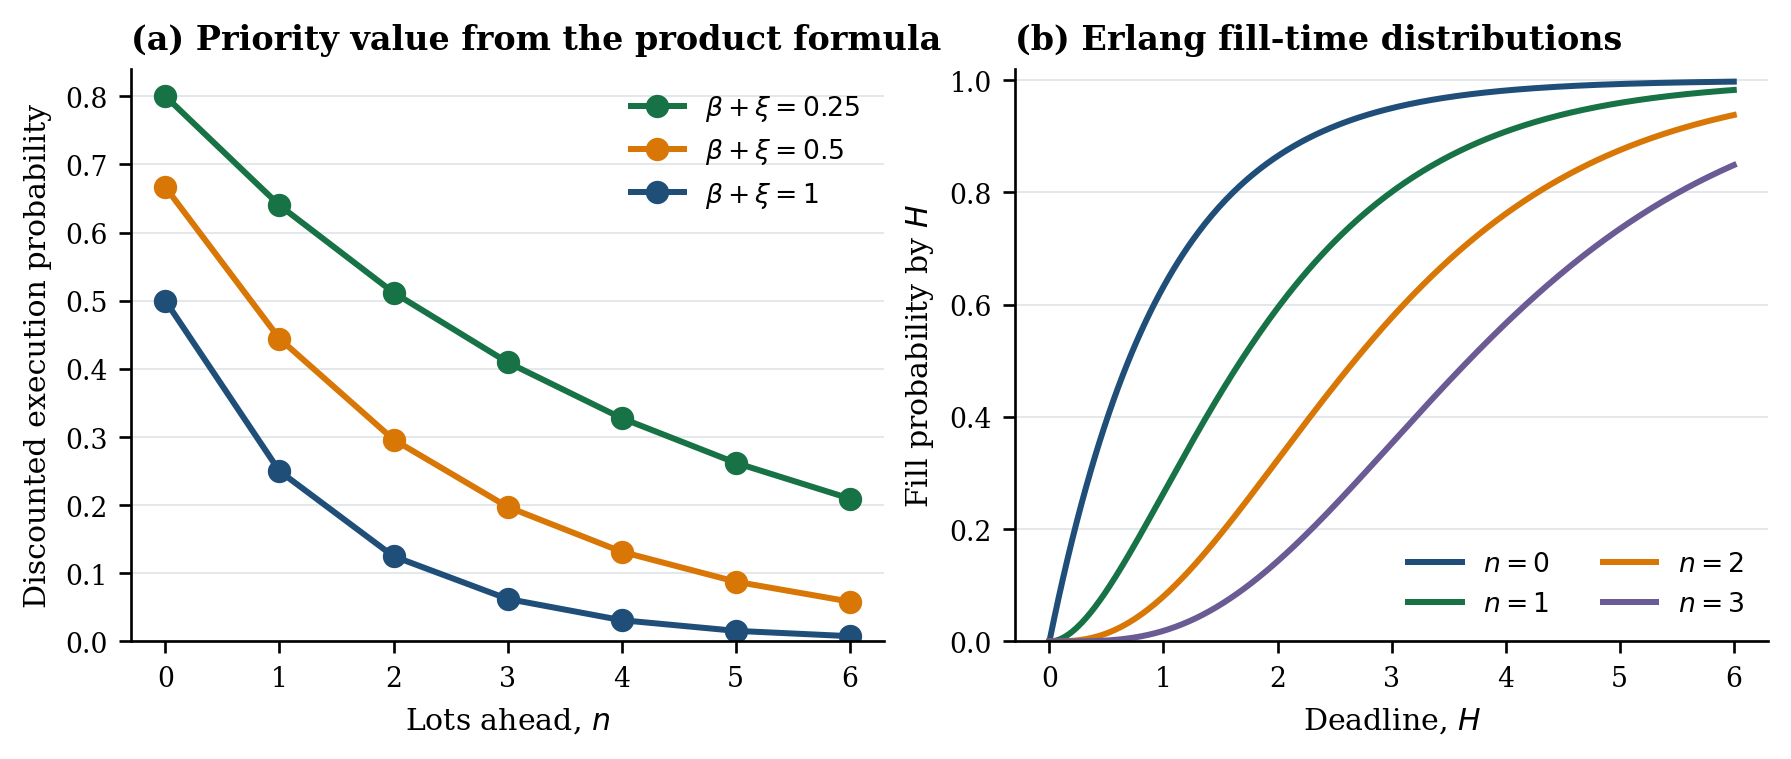
\includegraphics[width=\linewidth]{figures/01_queue_priority.png}
\caption{Queue priority in the tagged-order model. Panel (a) evaluates
\eqref{eq:queueproduct} with \(\mu=1\), no ahead cancellations, and three
values of \(\beta+\xi\); every extra lot ahead contributes another factor
\(\mu/(\mu+\beta+\xi)\). Panel (b) gives the exact Erlang fill
probabilities by deadline for ranks \(n=0,1,2,3\). These are analytic model
evaluations, not estimates from market data.}
\label{fig:queuepriority}
\end{figure}

\subsection{Batch consumption, partial fills, and marked volume}
\label{sec:partialfills}

A unit-order absorption model does not determine the fill distribution
of a larger tagged order. Let \(n\) lots be ahead of a tagged order
with \(m\) lots remaining. An aggressive event consuming \(B\)
lots at this price executes
\begin{equation}\label{eq:batchmatching}
 f=\min\{m,(B-n)_+\},\qquad
 n'=(n-B)_+,\qquad m'=m-f,\qquad q'=q+sf,
\end{equation}
where \(s=+1\) for a bid and \(s=-1\) for an ask.
The residual order retains its priority after a partial fill in
this price--time cell. An ahead cancellation removes ahead lots
without executing the tagged order. Rules that requeue the residual
quantity require a different state map.

For a bid, \(q'+m'=q+m\); for an ask, \(q'-m'=q-m\).
Consequently a valid reservation remains valid after any partial
fill, including a batch that exhausts the order. A pending cancel
retains the unfilled reservation \(m'\) until acknowledgement.
At acknowledgement only the remaining quantity is withdrawn:
executed inventory is not reversed.

Let \(\delta\) be the per-lot offset and \(J\) the simultaneous
reference-price jump. The complete jump in marked wealth is
\[
 \Delta W=\delta f+(q+sf)J.
\]
When carried inventory is already accounted for through its
total price compensator, the event's additional fill reward is
\(\delta f+sfJ\). Thus its expected contribution includes
\(\E[fJ\mid x,e]\). Multiplying expected fill volume by an
unconditional mean mark generally omits the dependence of price
selection on the size of the consuming event.

\begin{proposition}[A partial-fill transform]
\label{prop:partialfilltransform}
In a finite event cell, event \(e\) at state \(x\) has rate
\(\lambda_e(x)\), destination \(T_e(x)\), and integer executed
volume \(f_e(x)\ge0\). Track a fixed tagged order, with no
submission of additional tagged volume, and make cancellation
and full execution absorbing for its fill count. Let \(C_t\)
be its cumulative executed volume. For \(z\ge0\), define
\[
 (\mathcal Q_z u)_x
 =\sum_e\lambda_e(x)
       \{z^{f_e(x)}u_{T_e(x)}-u_x\},
 \qquad 0^0:=1.
\]
Then
\begin{equation}\label{eq:partialfillpgf}
 \E_x[z^{C_t}]=(e^{t\mathcal Q_z}\mathbf1)_x .
\end{equation}
In particular, the coefficients give the complete partial-fill
distribution, and derivatives at \(z=1\) give its factorial
moments. For a bounded expected marked-reward rate
\(r_x=\sum_e\lambda_e(x)\E[g_e\mid x,e]\), the expected
discounted cumulative event reward is
\begin{equation}\label{eq:partialfillreward}
 \E_x\!\left[\sum_{s\le t}e^{-\beta s}g_s\right]
 =\left[\int_0^t e^{s(\mathcal Q_1-\beta I)}r\dd s\right]_x .
\end{equation}
\end{proposition}
\begin{proof}
Condition on the first infinitesimal time interval. No event leaves
the transform unchanged; an event contributes the factor
\(z^{f_e(x)}\) and the continuation transform at \(T_e(x)\).
The resulting backward equation is
\(\partial_t u=\mathcal Q_z u,\ u(0)=\mathbf1\), proving
\eqref{eq:partialfillpgf}. The bounded tagged volume makes its
generating function a polynomial, justifying differentiation.
For the reward identity, the compensation formula gives the
integral of the state-dependent expected reward rate.
The state transition semigroup is \(e^{t\mathcal Q_1}\).
\end{proof}

State-preserving events must retain their factor
\(z^{f_e}\) in the tilted operator if they execute volume.
At \(z=1\), the operator is the ordinary generator, and
state-preserving terms cancel there as required.

\begin{corollary}[Compound-Poisson consumption]
\label{cor:compoundfills}
Suppose aggressive arrivals form a rate-\(\lambda\) Poisson process,
their independent positive integer sizes are \(B_1,B_2,\ldots\),
and ahead cancellations and invalidation are absent. With
\(S_t=\sum_{i=1}^{N_t}B_i\), a tagged order initially at
\((n,m)\) satisfies
\[
 C_t=\min\{m,(S_t-n)_+\},\qquad
 \mathbb P(C_t\ge j)=\mathbb P(S_t\ge n+j),\quad 1\le j\le m.
\]
Consequently
\(\E C_t=\sum_{j=1}^m\mathbb P(S_t\ge n+j)\).
If
\[
 k_*=\min\{k\ge1:\mathbb P(B_1+\cdots+B_k\ge n+1)>0\},
\]
then, as \(t\downarrow0\),
\[
 \mathbb P(C_t>0)=
 \frac{\lambda^{k_*}}{k_*!}
 \mathbb P(B_1+\cdots+B_{k_*}\ge n+1)t^{k_*}
 +O(t^{k_*+1}).
\]
\end{corollary}
\begin{proof}
Consumption first removes all ahead volume and then executes the
tagged order, giving the pathwise identity. The tail-sum formula
gives its mean. In the Poisson mixture for the first-fill probability,
all counts below \(k_*\) have zero contribution. The first nonzero
term has the stated coefficient, and the probability of more than
\(k_*\) arrivals is \(O(t^{k_*+1})\).
\end{proof}

For example, let \(n=3,m=2,\lambda=1.4\), with
\(\mathbb P(B=1)=0.7,\mathbb P(B=3)=0.3\). At least two events
are needed, and
\(\mathbb P(B_1+B_2\ge4)=0.51\). Hence
\[
 \mathbb P(C_t>0)=\frac{2499}{5000}t^2+O(t^3).
\]
A constant positive tagged-fill hazard would instead have a
linear leading term. Matching expected consumed volume
\(\lambda\E B\) does not repair this mismatch in short-latency
exposure.


\subsection{Cancellation and replacement at decision opportunities}

A continuously adjustable offset does not by itself model the loss
of time priority when an order is replaced. To keep messages within
the finite-rate framework, introduce an independent decision clock
of rate \(\nu\). At an opportunity, message \(b\) maps the current
book state to \(R_b(x)\), with immediate fee \(c_x(b)\ge0\).
The finite menu contains a no-op with \(R_0(x)=x,c_x(0)=0\).
All maps preserve \eqref{eq:inventoryreservation}. Between decision
opportunities the posted quote and tagged rank are state variables.

\begin{proposition}[A verified quote-replacement model]
\label{prop:replacementclock}
Let \(L^0,r^0\) describe bounded external book events and their
marked reward. The finite-horizon value satisfies
\begin{equation}\label{eq:replacementhjb}
\partial_t h_x+r_x^0+(L^0h)_x
 +\nu\max_b\{h_{R_b(x)}-h_x-c_x(b)\}=0,
\qquad h_x(T)=-\Phi_x.
\end{equation}
It has the verification and performance-difference identity of
Theorem~\ref{thm:verification}. In particular, a proposed replacement
is compared with keeping the existing order through its entire
post-message continuation value, including its new rank.
\end{proposition}
\begin{proof}
For a fixed message choice, the clock contributes generator
\(\nu[u_{R_b(x)}-u_x]\) and expected fee rate \(-\nu c_x(b)\).
Thus its Hamiltonian is
\(r_x^0+(L^0u)_x+\nu[u_{R_b(x)}-u_x-c_x(b)]\).
The finite action menu and bounded coefficients satisfy the hypotheses
of Theorem~\ref{thm:verification}. Taking the maximum over the menu
gives \eqref{eq:replacementhjb}, and the same Dynkin argument gives
the performance identity.
\end{proof}

An accepted atomic replacement is the message convention in this
model. If cancellation and insertion have separate delays, the state
must include the pending stages and permit fills of the still-live
order. Finite exponential stages provide another finite-state model;
a deterministic delay generally requires an additional age variable.
Neither model allows free continuous relocation while retaining the
old queue position. Discrete message choices use value-gap or hybrid
certificates; smooth offset curvature is not a property of a tick grid.

\subsection{Live orders during cancellation latency}
\label{sec:cancellatency}

A decision opportunity and an exchange acknowledgement are different
times. Latency and adverse selection in limit-order control are
already studied by \citet{LehalleMounjid2017}. The comparison here
concerns the error made when a specified pending-message delay is
replaced by an instantaneous reset or by finitely many exponential
stages.

After sending a cancellation, let \(X\) be the finite state of the
still-live book and tagged order, with generator \(Q\), until
acknowledgement. The state includes remaining quantity and all
inventory changes from partial fills. Further messages are suspended
during this pending period. Let \(r\) be its expected marked-reward
rate, including running inventory cost, and let \(w_x\) be the value
after acknowledging the cancellation from pre-acknowledgement state
\(x\). Thus \(w\) withdraws only the residual order and retains
the inventory actually accumulated. The acknowledgement delay
\(D\ge0\) has a common law across initial states, is independent
of future book events, and has finite mean. No independence of
fill size and price mark is required.

\begin{theorem}[The value and perturbation of a pending cancellation]
\label{thm:cancellationvalue}
For \(\beta\ge0\), put \(A=Q-\beta I\) and \(g=r+Aw\).
The value of the pending period and its continuation is
\begin{align}
 V^D&=\E\left[\int_0^D e^{tA}r\dd t+e^{DA}w\right],
 \label{eq:cancelvalue}\\
 V^D-w&=\E\int_0^D e^{tA}g\dd t .
 \label{eq:cancelresidual}
\end{align}
In particular, with \(G=\|g\|_\infty\),
\[
 \|V^D-w\|_\infty
 \le G\,\E\int_0^D e^{-\beta t}\dd t
 \le G\,\E D.
\]
For two independent-delay laws with finite first moments,
\begin{equation}\label{eq:delaywasserstein}
 \|V^D-V^{D'}\|_\infty
 \le G\,W_1(\mathcal L(D),\mathcal L(D')),
\end{equation}
where \(W_1\) is the minimum of \(\E|D-D'|\) over couplings
of their marginal delay laws.
\end{theorem}
\begin{proof}
Condition on the delay. The finite-state reward and terminal-value
formulas give \eqref{eq:cancelvalue}. Differentiation in a deterministic
delay \(t\) yields
\[
 \frac{\dd}{\dd t}
 \left\{\int_0^t e^{sA}r\dd s+e^{tA}w\right\}
 =e^{tA}(r+Aw)=e^{tA}g.
\]
Integrating from zero proves \eqref{eq:cancelresidual}. The
discounted Markov semigroup satisfies
\(\|e^{tA}\|_{\infty\to\infty}\le e^{-\beta t}\).
This proves the first bound and makes the deterministic-delay
value \(G\)-Lipschitz in time. Apply that Lipschitz inequality to
any coupling of \(D,D'\), take expectations, and then minimize
over couplings.
\end{proof}

The sign of \(g\) is not fixed. Delay can admit a profitable fill
or a damaging fill, change the inventory penalty, and discount the
post-acknowledgement continuation. A latency allowance must retain
those channels. If congestion makes the delay dependent on future
order flow, its marginal distribution does not determine
\eqref{eq:cancelvalue}; the joint state and acknowledgement law
must be modeled.

\begin{theorem}[A sharp finite-stage approximation of deterministic latency]
\label{thm:erlanglatency}
In Theorem~\ref{thm:cancellationvalue}, fix \(d>0\) and replace the
deterministic delay \(d\) by an independent Erlang delay \(D_k\)
with \(k\) stages of rate \(\kappa=k/d\). Let
\[
 B=\|Ag\|_\infty,\qquad C=\|A^2g\|_\infty.
\]
The finite-stage value is computed by
\begin{equation}\label{eq:erlangrecursion}
 v_0=w,\qquad
 [(\kappa+\beta)I-Q]v_j=r+\kappa v_{j-1},
 \quad j=1,\ldots,k,\qquad V^{D_k}=v_k .
\end{equation}
It satisfies the uniform bounds
\begin{equation}\label{eq:erlangweakbound}
 \|V^{D_k}-V^d\|_\infty
 \le\min\left\{\frac{Gd}{\sqrt{k}},\frac{Bd^2}{2k}\right\},
\end{equation}
and the explicit expansion
\begin{equation}\label{eq:erlangexpansion}
 \left\|V^{D_k}-V^d-
          \frac{d^2}{2k}e^{dA}Ag\right\|_\infty
 \le \frac{Cd^3}{6k^{3/2}}\sqrt{3+\frac6k}.
\end{equation}
The order \(k^{-1}\) in \eqref{eq:erlangweakbound} cannot be
improved uniformly over finite queue cells.
\end{theorem}
\begin{proof}
Conditioning on the first exponential stage gives the resolvent
equation \eqref{eq:erlangrecursion}. Its inverse exists because
\(\kappa+\beta>0\) and \(Q\) is a finite generator.
The Erlang law has mean \(d\) and variance \(d^2/k\).
The Wasserstein bound against the constant \(d\), followed by
Cauchy--Schwarz, gives the first term in \eqref{eq:erlangweakbound}.

Write the deterministic-delay value as \(f(t)\). The preceding
proof gives \(f'(t)=e^{tA}g\),
\(f''(t)=e^{tA}Ag\), and \(f'''(t)=e^{tA}A^2g\).
Their sup-norm bounds are respectively \(G,B,C\).
Taylor expansion about \(d\), with
\(\E(D_k-d)=0\), gives the second bound. Keeping the second-order
term gives the leading vector in \eqref{eq:erlangexpansion}.
The absolute third-order remainder is bounded using
\begin{align*}
 \E|D_k-d|^3
 &\le\{\E(D_k-d)^2\,\E(D_k-d)^4\}^{1/2},\\
 \E(D_k-d)^4&=\frac{3d^4}{k^2}+\frac{6d^4}{k^3}.
\end{align*}
These identities give the displayed remainder.

For sharpness, place one tagged unit at the front of a queue,
with fill rate \(\mu>0\), positive fill reward \(R\), no other
reward, and zero post-cancellation value. Until acknowledgement
the unit remains executable. Then
\[
 V^d=\frac{\mu R}{\mu+\beta}(1-e^{-(\mu+\beta)d}),\qquad
 V^{D_k}=\frac{\mu R}{\mu+\beta}
       \{1-(1+(\mu+\beta)d/k)^{-k}\}.
\]
Expanding the logarithm shows
\[
 k(V^{D_k}-V^d)\longrightarrow
 -\frac{\mu R(\mu+\beta)d^2}{2}e^{-(\mu+\beta)d}\ne0.
\]
Thus a genuine tagged-fill example attains the stated order.
\end{proof}

The first bound only uses control of the random time displacement.
Matching the mean cancels its linear contribution to the expected
value, which explains the sharper \(k^{-1}\) rate. This is a bound
on value approximation, not on pathwise proximity of acknowledgement
times. Known stage-approximation allowances can be added to local
message-value intervals. For a finite menu of one-time message
choices with uniform error \(\zeta\), choosing the best approximate
value loses at most \(2\zeta\), by the same two-value comparison
as Corollary~\ref{cor:queueperturbation}.


\subsection{From event-law errors to Hamiltonian error budgets}

The event representation makes the primitive bounds used below traceable
to the book model. Fix a smooth action branch on which the event maps
\(T_e(x)\) agree in the true and estimated models. If the destination of
an event is uncertain, index channels by both event type and destination
and put the uncertainty in their rates. Moving a destination without
recording that change in the rates is outside this comparison.

\begin{proposition}[Event-law derivative budgets]
\label{prop:eventbudgets}
Suppose the rates, conditional mean rewards, and base rewards in
\eqref{eq:eventreward} have derivatives through order two on the branch.
For \(j=0,1,2\), let uniform bounds satisfy
\begin{align*}
 \sum_e\norm{D^j(\lambda_e-\widehat\lambda_e)}
 &\le\varepsilon_{\lambda,j},&
 \sup_e\norm{D^j(g_e-\widehat g_e)}
 &\le\varepsilon_{g,j},\\
 \norm{D^j(c-\widehat c)}&\le\varepsilon_{c,j},&
 \sup_e\norm{D^jg_e}&\le G_j,\\
 \sum_e\norm{D^j\widehat\lambda_e}
 &\le\widehat L_{\lambda,j}.&&
\end{align*}
Here order zero means absolute value and higher orders use the
corresponding operator norms. The off-diagonal transition rates
\(k_{xy}=\sum_{e:T_e(x)=y}\lambda_e\), \(y\ne x\), and running rewards obey
\begin{align}
 \sum_{y\ne x}\norm{D^j(k_{xy}-\widehat k_{xy})}
 &\le\varepsilon_{\lambda,j},\label{eq:eventratebudget}\\
 \norm{D^j(r-\widehat r)}
 &\le\varepsilon_{c,j}
 +\sum_{\ell=0}^{j}\binom{j}{\ell}
 \left(G_{j-\ell}\varepsilon_{\lambda,\ell}
 +\widehat L_{\lambda,\ell}\varepsilon_{g,j-\ell}\right).
 \label{eq:eventrewardbudget}
\end{align}
\end{proposition}
\begin{proof}
Group the event rates by their common destination and apply the triangle
inequality. Omitting self-events cannot increase the bound in
\eqref{eq:eventratebudget}. For the reward, write
\[
 r-\widehat r=c-\widehat c
 +\sum_e\big[(\lambda_e-\widehat\lambda_e)g_e
             +\widehat\lambda_e(g_e-\widehat g_e)\big].
\]
Apply the product rule. At order two, the two cross terms are outer
products whose operator norms are bounded by the products of the
gradient norms. Taking norms and using the displayed bounds gives
\eqref{eq:eventrewardbudget} at each order.
\end{proof}

Order zero supplies the value-error budget. Order one supplies the
gradient discrepancy, and order two supplies the curvature enclosure
in Section~\ref{sec:computed}. The quantities \(G_j\) can themselves be
bounded by fitted derivatives plus the corresponding uncertainty
bound. These are assumptions or certified enclosures, not consequences
of observing a finite sample. The \(g_e\) are conditional means;
the proposition does not assume that every realized price mark is
bounded. A derivative certificate applies within a fixed smooth
branch. Queue resets, participation changes, and ticks require the
finite-action or hybrid comparison below.

\subsection{The cost of truncating the book}

A finite depth cap changes the model when the book reaches its
boundary. The following comparison separates that error from
parameter estimation and numerical solution.

\begin{proposition}[A coupling certificate for a finite cell]
\label{prop:booktruncation}
Suppose a nonexplosive full book and a capped book can be coupled to
have identical states, feasible actions, and rewards up to the first
exit time \(\tau\) from their common retained cell. Policies on the two
models correspond before exit and admit feasible extensions after exit.
Terminal payoffs agree within the retained cell.
Assume \(|r|\le R_\infty\) and \(|\Phi|\le\Phi_\infty\) in both models.
For any corresponding policy pair, started at \((t,x)\) inside the cell,
\begin{equation}\label{eq:capfixedpolicy}
 |J_{\rm full}^{\pi}-J_{\rm cap}^{\pi}|
 \le 2\E\!\left[\mathbf1_{\{\tau\le T\}}
       \{\Phi_\infty+R_\infty(T-\tau)\}\right]
 \le 2B(t)\,\mathbb P(\tau\le T),
\end{equation}
where \(B(t)=\Phi_\infty+R_\infty(T-t)\).
If the exit probability is at most \(p\) uniformly over the compared
policy class, then
\begin{equation}\label{eq:capoptimal}
 |V_{\rm full}-V_{\rm cap}|\le2B(t)p.
\end{equation}
A policy with regret at most \(C\) in the capped model therefore has
regret at most \(C+4B(t)p\) in the full model.
\end{proposition}
\begin{proof}
The pathwise reduced rewards coincide before exit, and the complete
payoffs coincide on \(\{\tau>T\}\). On exit, the difference between the
remaining integrated rewards is at most \(2R_\infty(T-\tau)\), and the
terminal difference is at most \(2\Phi_\infty\). Taking expectations
gives \eqref{eq:capfixedpolicy}. Uniformity and policy correspondence
permit taking suprema, which proves \eqref{eq:capoptimal}. Finally,
insert the capped optimal value and the capped deployed-policy value
between the corresponding full-model values. The two comparison
errors are each at most \(2B(t)p\), and the middle gap is at most \(C\).
\end{proof}

The uniform exit bound must cover the deployed policy and the policies
against which it is compared. A small boundary frequency under a
logging policy alone does not establish it. Reward bounds and feasible
post-exit extensions are also substantive assumptions. This result
allows the finite-cell certificates to be used with an explicit
truncation allowance; it does not justify an arbitrary replenishment
rule from the fact that the retained state space is finite.

\section{Offsets, inventory shadow values, and selection effects}

Consider one active side at a fixed state and time. Suppose its
Hamiltonian contribution can be written
\[
R(\delta)=(\delta-p)\Lambda(\delta),
\]
where \(p\in\R\) is independent of the offset. For a fill leaving the
market state unchanged and having conditional mean jump \(m_s\),
\[
p=h_{q,z}(t)-h_{q+\epsilon_s,z}(t)-\epsilon_s m_s.
\]
An inventory-reducing fill can have negative shadow cost, so \(p\) is
not restricted to be nonnegative.

\begin{proposition}[The quote equation]\label{prop:quote}
Let \(\Lambda>0\) be continuously differentiable and decreasing.
At an interior maximizer with \(\Lambda'(\delta^\ast)<0\),
\[
\delta^\ast=p-\frac{\Lambda(\delta^\ast)}{\Lambda'(\delta^\ast)}.
\]
For \(\Lambda(\delta)=\Lambda_0e^{-\kappa\delta}\), the maximizer
on \([0,D]\) is
\[
\delta^\ast=\min\{D,\max\{0,p+1/\kappa\}\}.
\]
If withdrawal is allowed, compare the resulting Hamiltonian contribution
with the value zero of an inactive side.
\end{proposition}
\begin{proof}
Differentiate \(R\). For the exponential law,
\(R'=\Lambda_0e^{-\kappa\delta}[1-\kappa(\delta-p)]\), whose sign changes
at most once, from positive to negative. Clipping its unconstrained
maximizer to the interval proves the assertion. Withdrawal is a separate
feasible action.
\end{proof}

The exponential objective is not globally concave:
\[
R''(\delta)=
\Lambda_0e^{-\kappa\delta}
\big[\kappa^2(\delta-p)-2\kappa\big].
\]
Strong-concavity certificates below apply only on regions on which this
second derivative has a uniform negative upper bound.
Also, the usual demand elasticity is
\(-\delta\Lambda'/\Lambda=\kappa\delta\), which is not constant.
The constant object is the inverse semi-elasticity
\(-\Lambda/\Lambda'=1/\kappa\).

\begin{proposition}[Offset-dependent adverse selection]\label{prop:selection}
If the expected mark or continuation value conditional on a fill depends
on the offset, write \(R(\delta)=(\delta-p(\delta))\Lambda(\delta)\).
For differentiable \(p\), an interior optimum satisfies
\[
0=(1-p'(\delta^\ast))\Lambda(\delta^\ast)
 +(\delta^\ast-p(\delta^\ast))\Lambda'(\delta^\ast).
\]
Thus a fixed markup plus a fixed shadow cost is valid only when the
relevant conditional penalty is offset-independent.
\end{proposition}
\begin{proof}
This is the product rule applied to \(R\).
\end{proof}

In the exponential-utility model of \citet{AvellanedaStoikov2008}, the
intensity contribution is
\(\gamma^{-1}\log(1+\gamma/\kappa)\), approaching \(1/\kappa\) as
\(\gamma\downarrow0\). The exact utility objective matters; the
risk-neutral Hamiltonian above does not make all risk-aversion
specifications equivalent.

\section{An exact gross-profit shutdown threshold}

\begin{definition}[Two populations]\label{def:populations}
On one ask side, uninformed fills arrive at rate
\(\lambda_u e^{-\kappa\delta}\), with \(\lambda_u,\kappa>0\), and have
zero expected per-fill markout. Informed opportunities arrive at rate
\(\lambda_i\ge0\). Their upward mark \(J\) is exponential with parameter
\(k>0\); a trader fills the ask precisely when \(J>\delta\).
The objective in this section is the sum of incremental per-fill
markouts, excluding pre-existing inventory, fees, and continuation value.
\end{definition}

Memorylessness gives
\(\E[J-\delta\mid J>\delta]=1/k\).
Consequently the per-time gross markout is
\begin{equation}\label{eq:shutdownreward}
g(\delta)=\lambda_u\delta e^{-\kappa\delta}
             -\frac{\lambda_i}{k}e^{-k\delta}.
\end{equation}
This is a static component of a quoting objective; it is not a theorem
that the entire dynamic inventory book should be shut down.

\begin{theorem}[Unbounded-offset threshold]\label{thm:shutdown}
For the objective \eqref{eq:shutdownreward} on \(\delta\ge0\):
\begin{enumerate}
\item If \(k\ge\kappa\), some finite offset has strictly positive
gross profit, for every finite \(\lambda_i\).
\item If \(k<\kappa\), every offset has nonpositive gross profit if and
only if
\[
\lambda_i\ge\lambda_i^\ast:=
\frac{k\lambda_u}{e(\kappa-k)}.
\]
At equality the only zero at finite offset is
\(\delta=1/(\kappa-k)\).
\end{enumerate}
\end{theorem}
\begin{proof}
Multiplication by \(e^{k\delta}\) shows that \(g(\delta)>0\) is equivalent
to
\(\lambda_u\delta e^{-(\kappa-k)\delta}>\lambda_i/k\).
For \(k\ge\kappa\) the left side is unbounded. For \(k<\kappa\) its
unique maximum is \(\lambda_u/[e(\kappa-k)]\), at the stated offset.
\end{proof}

\begin{corollary}[A finite quote range]\label{cor:finitequote}
On \([0,D]\), \(D>0\), a positive quote exists if and only if
\[
\lambda_i<
k\lambda_u\max_{0\le\delta\le D}
\delta e^{-(\kappa-k)\delta}.
\]
The maximizing offset in this expression is
\(\min\{D,1/(\kappa-k)\}\) if \(k<\kappa\), and \(D\) if
\(k\ge\kappa\).
\end{corollary}
\begin{proof}
Apply the same inequality on the compact feasible interval.
\end{proof}

Heavier informed tails correspond to \(k<\kappa\), precisely the regime
where the unbounded-offset shutdown threshold exists. On a finite quote
range there is a threshold in both regimes. At a hard inventory limit,
withdrawal may be mandatory independently of these profitability
comparisons. A fill that reduces a sufficiently costly inventory can also
have positive continuation value despite a negative immediate markout.

\begin{example}[Threshold arithmetic]
With \(\lambda_u=10,\kappa=2,k=1\), the threshold is
\(10/e\approx3.678794\), attained at \(\delta=1\).
At \(\lambda_i=10/e\), the two terms of \(g(1)\) both equal
\(10e^{-2}\). Values \(\lambda_i<10/e\) leave a profitable interval;
values above it make all finite quotes unprofitable for this static
criterion.
\end{example}

Figure~\ref{fig:shutdown} makes the phase boundary in
Theorem~\ref{thm:shutdown} explicit.

\begin{figure}[tbp]
\centering
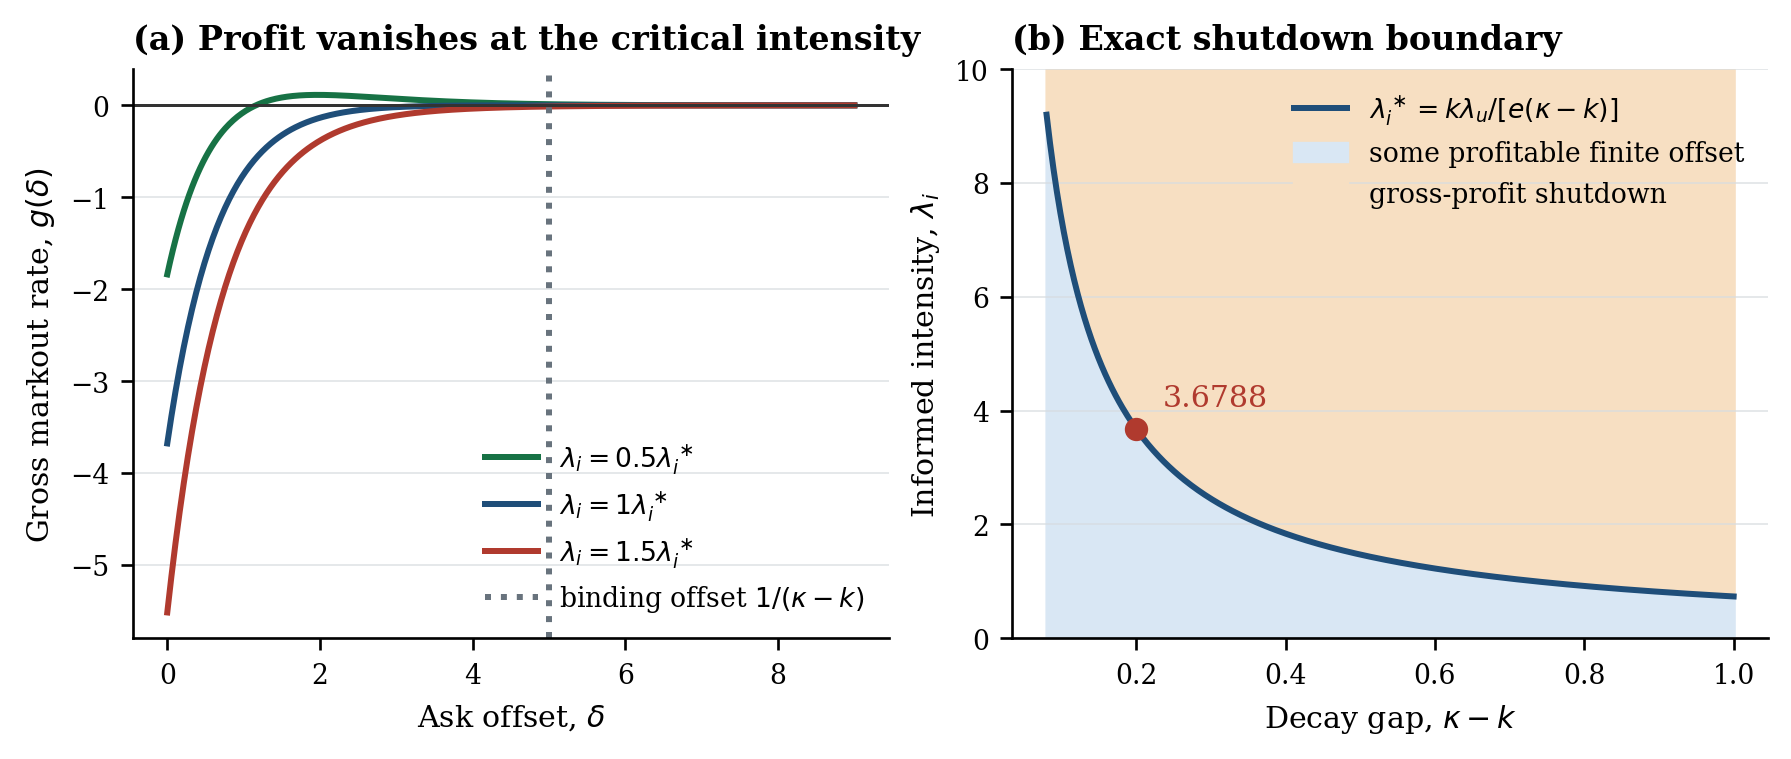
\includegraphics[width=\linewidth]{figures/02_shutdown_threshold.png}
\caption{Exact gross-profit shutdown geometry. Panel (a) plots
\(g(\delta)\) for \(\lambda_u=2\), \(\kappa=1.2\), \(k=1\), and informed
intensities equal to one half, exactly, and one and a half times the
critical value. At equality the maximum is zero at
\(\delta=1/(\kappa-k)=5\). Panel (b) plots
\(\lambda_i^*=k\lambda_u/[e(\kappa-k)]\); the red point is the threshold
\(10/e\) from the arithmetic example. The shaded regions indicate whether
some finite offset has positive gross markout under the stated static
criterion.}
\label{fig:shutdown}
\end{figure}

\section{Certificates for a misspecified quoting model}

\subsection{A constrained local certificate}

\begin{lemma}[Gradient error on a convex action set]\label{lem:local}
Let \(A\subset\R^d\) be convex and compact, and let \(F,\widehat F\)
be differentiable on a neighborhood of \(A\). Assume \(F\) is
\(m\)-strongly concave on \(A\), \(m>0\), and
\(a^\ast\in\arg\max_A F\), \(\widehat a\in\arg\max_A\widehat F\).
Then, including boundary maximizers,
\begin{align}
0\le F(a^\ast)-F(\widehat a)
&\le\frac{\norm{\nabla(F-\widehat F)(\widehat a)}^2}{2m},
\label{eq:local}\\
\norm{a^\ast-\widehat a}
&\le\frac{\norm{\nabla(F-\widehat F)(\widehat a)}}{m}.
\end{align}
\end{lemma}
\begin{proof}
Put \(d=a^\ast-\widehat a\).
The first-order necessary inequality for the constrained maximum of
\(\widehat F\) gives \(\nabla\widehat F(\widehat a)\cdot d\le0\).
Strong concavity therefore gives
\[
F(a^\ast)-F(\widehat a)
\le\nabla(F-\widehat F)(\widehat a)\cdot d-\frac m2\norm d^2
\le\frac{\norm{\nabla(F-\widehat F)(\widehat a)}^2}{2m}.
\]
For the distance bound, the optimality inequality for \(F\) at \(a^\ast\)
and strong monotonicity of \(-\nabla F\) imply
\[
m\norm d^2
\le(\nabla F(\widehat a)-\nabla F(a^\ast))\cdot d
\le\nabla(F-\widehat F)(\widehat a)\cdot d.
\]
Cauchy--Schwarz completes the proof.
\end{proof}

For a one-dimensional fixed-\(p\) reward
\(R=(\delta-p)\Lambda\), the residual is
\[
(R-\widehat R)'=
(\Lambda-\widehat\Lambda)
 +(\delta-p)(\Lambda'-\widehat\Lambda').
\]
A constant multiplicative intensity error leaves a fixed-\(p\) optimizer
unchanged. It need not leave the dynamic optimizer unchanged, because
the intensity scale changes the time available to adjust inventory and
therefore changes the value function.

\subsection{From a quote error to total policy regret}

Let \((\widehat r,\widehat k)\) be a second finite-state control model
with the same state set, action sets, and terminal penalty.
Its value and Hamiltonian are \(\widehat h,\widehat\HH\).
Let \(\widehat\pi(t,x)\) maximize
\(\widehat\HH_x(a;\widehat h(t))\).
Define
\[
e_x(t,a)=
\HH_x(a;h(t))-\widehat\HH_x(a;\widehat h(t)).
\]
This error includes the difference in continuation values. Holding
\(h\) fixed while replacing the fill law would omit a policy-relevant
part of the misspecification.

\begin{theorem}[Dynamic gradient certificate]\label{thm:dynamiccertificate}
Suppose each \(\cAct_x\) is a common convex compact quote region,
the two Hamiltonians are differentiable in \(a\), and
\(\HH_x(\cdot;h(s))\) is \(m_x(s)\)-strongly concave with
\(m_x(s)\ge m_0>0\). Then
\begin{equation}\label{eq:dynamic}
0\le h_x(t)-J^{\widehat\pi}(t,x)
\le\E^{\widehat\pi,\mathrm{true}}_{t,x}
\int_t^T
\frac{\norm{\nabla_a e_{X_s}(s,\widehat\pi(s,X_s))}^2}
{2m_{X_s}(s)}\dd s .
\end{equation}
In particular a uniform bound \(\norm{\nabla_a e_x(s,a)}\le b(s)\)
gives regret at most \(\int_t^T b(s)^2/(2m_0)\dd s\).
\end{theorem}
\begin{proof}
Use Lemma~\ref{lem:local} at each time and state with
\(F=\HH_x(\cdot;h(s))\) and
\(\widehat F=\widehat\HH_x(\cdot;\widehat h(s))\).
Substitute its gap bound in \eqref{eq:performance}.
The expectation is under the true controlled process, exactly as in the
performance identity; no equality of visitation laws is assumed.
\end{proof}

\subsection{Primitive errors and the continuation-value contribution}

Let \(\Phi_\infty=\max_x|\Phi_x|\), and assume both models' rewards are
bounded by \(R_\infty\). Put
\[
B(s)=\Phi_\infty+(T-s)R_\infty.
\]
Both value functions have sup norm at most \(B(s)\).
For simplicity write time-independent error budgets
\begin{align*}
\varepsilon_r&=\sup_{x,a}|r_x(a)-\widehat r_x(a)|,\\
\varepsilon_k&=\sup_{x,a}\sum_{y\ne x}|k_{xy}(a)-\widehat k_{xy}(a)|,\\
\varepsilon_{r,1}&=\sup_{x,a}\norm{\nabla r_x(a)-\nabla\widehat r_x(a)},\\
\varepsilon_{k,1}&=\sup_{x,a}\sum_{y\ne x}
\norm{\nabla k_{xy}(a)-\nabla\widehat k_{xy}(a)},\\
L_{k,1}&=\sup_{x,a}\sum_{y\ne x}\norm{\nabla\widehat k_{xy}(a)} .
\end{align*}
The gradients are taken within the common convex regions.

\begin{lemma}[Value-function perturbation]\label{lem:valueerror}
Under the finite-state assumptions,
\begin{equation}\label{eq:valueerror}
\norm{h(t)-\widehat h(t)}_\infty
\le d(t):=\int_t^T
\big[\varepsilon_r+2B(s)\varepsilon_k\big]\dd s .
\end{equation}
This estimate does not require concavity.
\end{lemma}
\begin{proof}
For \(u=\widehat h(s)\), the Hamiltonians at the same \(u\) differ
uniformly by at most
\(c(s)=\varepsilon_r+2B(s)\varepsilon_k\).
Adding a constant vector does not change any \(L^a u\).
Consequently \(\widehat h(s)+d(s)\mathbf1\) has terminal value
\(-\Phi\) and satisfies
\(\partial_s u+\max_a\HH(a;u)\le0\).
Dynkin's formula shows that it dominates every true-policy value.
The vector \(\widehat h(s)-d(s)\mathbf1\) satisfies the reverse
inequality; a true-Hamiltonian maximizing selector for that vector
attains a value at least as large. This brackets \(h\) between the two
vectors and proves the bound.
\end{proof}

\begin{corollary}[A certificate in primitive model errors]\label{cor:primitive}
Under Theorem~\ref{thm:dynamiccertificate} and the displayed budgets,
one may take
\[
b(s)=\varepsilon_{r,1}
       +2B(s)\varepsilon_{k,1}
       +2d(s)L_{k,1}
\]
in \eqref{eq:dynamic}.
If the four error budgets are \(O(\varepsilon)\) and the horizon,
reward bounds, derivative bounds, and \(m_0^{-1}\) remain bounded,
the policy regret is \(O(\varepsilon^2)\).
\end{corollary}
\begin{proof}
Expand the gradient of \(e_x\) as
\begin{align*}
\nabla e_x={}&\nabla(r_x-\widehat r_x)
 +\sum_{y\ne x}\nabla(k_{xy}-\widehat k_{xy})(h_y-h_x)\\
&+\sum_{y\ne x}\nabla\widehat k_{xy}
\big[(h_y-\widehat h_y)-(h_x-\widehat h_x)\big].
\end{align*}
The differences in the first sum have magnitude at most \(2B(s)\);
those in the second at most \(2d(s)\), by Lemma~\ref{lem:valueerror}.
The triangle inequality gives the bound on \(b\).
The rate statement follows with a fixed positive concavity modulus.
\end{proof}

The budgets must be justified on the region used by the policy.
A fitted kernel and a fitted Hessian alone do not certify their errors
relative to the true market. For random estimates, simultaneous
high-probability bounds on these quantities give a certificate on the
same event. Constants deteriorate near flat Hamiltonians and near an
uncontrolled increase of the horizon.

\subsection{Withdrawal, ticks, and branch changes}

\begin{proposition}[A value-error certificate without concavity]\label{prop:switch}
On any compact action set, possibly disconnected or finite, suppose
\[
\sup_{a\in\cAct_x}
|\HH_x(a;h(s))-\widehat\HH_x(a;\widehat h(s))|
\le\zeta_x(s).
\]
The estimated maximizer has true Hamiltonian gap at most \(2\zeta_x(s)\).
Therefore its dynamic regret is at most
\(\E^{\widehat\pi,\mathrm{true}}\int_t^T2\zeta_{X_s}(s)\dd s\).
\end{proposition}
\begin{proof}
Let \(a^\ast\) maximize the true Hamiltonian. Insert the estimated
Hamiltonian at \(a^\ast\) and at \(\widehat a\). Its optimality gives
\(\widehat\HH(a^\ast)\le\widehat\HH(\widehat a)\), leaving at most
two uniform errors. Apply \eqref{eq:performance}.
\end{proof}

If action branches represent different active sides, a true gap
strictly larger than \(2\zeta_x(s)\) between the best branch and every
other branch preserves the selected branch. A local quadratic
certificate then applies if that branch is convex and strongly concave.
Without such a margin, branch switching prevents a universal quadratic
bound based only on a within-branch gradient. Tick-constrained quotes
are governed by the value-error bound unless an additional discrete
decision margin is established.

\subsection{Stationary discounting and the effective horizon}

Suppose the primitives are stationary and satisfy
Assumption~\ref{ass:finite}; there is no terminal penalty. For a discount
rate \(\beta>0\), define
\[
J_\beta^\pi(x)=\E_x^\pi\int_0^\infty e^{-\beta s}
 r_{X_s}(a_s)\dd s,\qquad h_x=\sup_\pi J_\beta^\pi(x).
\]
Take a second stationary model with the same state and action sets,
both rewards bounded by \(R_\infty\), and the primitive budgets above.
Let \(\overline K\) bound the total exit rates of both models, and put
\begin{align}
B_\beta&=R_\infty/\beta,\qquad
d_\beta=(\varepsilon_r+2B_\beta\varepsilon_k)/\beta,\notag\\
b_\beta&=\varepsilon_{r,1}+2B_\beta\varepsilon_{k,1}
                         +2d_\beta L_{k,1}.\label{eq:discountbudgets}
\end{align}

\begin{theorem}[Discounted policy certificate]\label{thm:discounted}
The equation \(\beta h_x=\max_{a\in\cAct_x}\HH_x(a;h)\) has a unique
solution. It is the discounted value, and a maximizing stationary
selector is optimal. Every admissible policy satisfies
\begin{equation}\label{eq:discountperformance}
h_x-J_\beta^\pi(x)=\E_x^\pi\int_0^\infty e^{-\beta s}
 \left[\max_{a\in\cAct_{X_s}}\HH_{X_s}(a;h)
                         -\HH_{X_s}(a_s;h)\right]\dd s.
\end{equation}
Moreover \(\norm h_\infty,\norm{\widehat h}_\infty\le B_\beta\) and
\(\norm{h-\widehat h}_\infty\le d_\beta\).
If the common action sets are convex and compact, both Hamiltonians
are differentiable in the actions, and every true
\(\HH_x(\cdot;h)\) is \(m_0\)-strongly concave, \(m_0>0\), then the
stationary estimated optimal policy obeys
\begin{equation}\label{eq:discountregret}
0\le h_x-J_\beta^{\widehat\pi}(x)
\le \frac{b_\beta^2}{2m_0\beta}\qquad\hbox{for every }x.
\end{equation}
\end{theorem}
\begin{proof}
Write \(k_x(a)=\sum_{y\ne x}k_{xy}(a)\). The uniformized operator
\[
(\mathcal Tu)_x=\frac{1}{\beta+\overline K}
\max_{a\in\cAct_x}\left[r_x(a)+\sum_{y\ne x}k_{xy}(a)u_y
                    +(\overline K-k_x(a))u_x\right]
\]
is a sup-norm contraction with factor
\(\overline K/(\beta+\overline K)<1\): its coefficients on \(u\)
are nonnegative and sum to \(\overline K\). Its fixed-point equation
is the displayed discounted HJB equation. This proves existence and
uniqueness. Discounted Dynkin's formula for the bounded vector \(h\),
followed by passage to the infinite horizon, gives
\[
h_x=J_\beta^\pi(x)+\E_x^\pi\int_0^\infty e^{-\beta s}
 [\beta h_{X_s}-\HH_{X_s}(a_s;h)]\dd s.
\]
The transversality term vanishes by boundedness. The bracket is
nonnegative and is zero under a maximizing selector, proving the
value assertion and \eqref{eq:discountperformance}.

The reward bound gives \(\norm h_\infty,\norm{\widehat h}_\infty
\le B_\beta\). At the common vector \(\widehat h\), the two
Hamiltonians differ by at most
\(c_\beta=\varepsilon_r+2B_\beta\varepsilon_k\).
Because generators annihilate constants, \(u^+=\widehat h+d_\beta\mathbf1\)
satisfies \(\beta u_x^+\ge\max_a\HH_x(a;u^+)\); discounted Dynkin's
formula shows \(u^+\ge h\). The reverse inequality holds for
\(u^-=\widehat h-d_\beta\mathbf1\). Under a selector maximizing
\(\HH(\cdot;u^-)\), the same formula gives
\(u^-\le J_\beta^\pi\le h\). This proves the perturbation bound.
The gradient expansion in Corollary~\ref{cor:primitive}, with
\(B_\beta,d_\beta\), bounds the full gradient error by \(b_\beta\).
Lemma~\ref{lem:local} bounds the bracket in
\eqref{eq:discountperformance} by \(b_\beta^2/(2m_0)\).
Integration of the discount factor proves \eqref{eq:discountregret}.
\end{proof}

\begin{remark}[Dependence on the discount rate]
The certificate has no terminal-horizon parameter, but its constants
are not uniform as \(\beta\downarrow0\). In fact
\[
b_\beta=\varepsilon_{r,1}
 +\frac{2R_\infty\varepsilon_{k,1}+2L_{k,1}\varepsilon_r}{\beta}
 +\frac{4R_\infty L_{k,1}\varepsilon_k}{\beta^2}.
\]
If all four error budgets are \(O(\varepsilon)\), with uniform
\(R_\infty,L_{k,1},m_0^{-1}\), the displayed bound is in general
\(O(\varepsilon^2\beta^{-5})\) as \(\beta\downarrow0\), and its
discount-normalized version is \(O(\varepsilon^2\beta^{-4})\).
These are growth rates of this upper bound, not matching lower bounds
on actual regret. The reward bound also gives
\(h_x-J_\beta^\pi(x)\le2R_\infty/\beta\), so the minimum with that
bound may always be taken. If the \(\beta^{-2}\) contribution to \(b_\beta\)
vanishes, for example when \(\varepsilon_k=0\), the corresponding
bounds improve to \(O(\varepsilon^2\beta^{-3})\) and
\(O(\varepsilon^2\beta^{-2})\). An ergodic limit requires additional
stability and relative-value analysis; it does not follow by setting
\(\beta=0\) here. The ergodic analysis of \citet{CaoEtAl2026} addresses
a different regime.
\end{remark}

\section{A certificate from computed values and supplied error bounds}
\label{sec:computed}

An exact estimated HJB solution is not a numerical output. A solver
returns an approximation, and a quoting routine can stop before reaching
its maximum. The following result keeps both errors in the certificate.
It also verifies curvature against model uncertainty.

Suppose the common action sets are compact and convex, and the
primitive rewards and rates are twice continuously differentiable on
their neighborhoods. Let \(v:[0,T]\to\R^{|\XX|}\) be a computed
continuation vector of class \(C^1\). Assume supplied, simultaneous
bounds, uniform over states and actions, for \(j=0,1,2\):
\[
\norm{\nabla^j(r-\widehat r)}\le\epsilon_{r,j},\qquad
\sum_{y\ne x}\norm{\nabla^j(k_{xy}-\widehat k_{xy})}
 \le\epsilon_{k,j}.
\]
For \(j=0\) the norm is absolute value; for \(j=2\) it is the matrix
operator norm. Bounds may depend on time. Let
\[
\overline K_j(s)\ge
\sup_{x,a}\sum_{y\ne x}\norm{\nabla^j\widehat k_{xy}(a)}
 +\epsilon_{k,j}(s),\qquad j=1,2.
\]
Thus \(\overline K_j\) also bounds the true rate derivatives.
Define the computed HJB and terminal residual bounds by
\[
\rho(s)\ge\max_x\left|
 \partial_s v_x(s)+\max_a\widehat\HH_x(a;v(s))\right|,
\qquad d_T\ge\norm{v(T)+\Phi}_\infty,
\]
and write \(\spn(v)=\max_xv_x-\min_xv_x\). Set
\begin{align}
c(s)&=\epsilon_{r,0}(s)+\spn(v(s))\epsilon_{k,0}(s),\notag\\
D(t)&=d_T+\int_t^T[\rho(s)+c(s)]\dd s,\label{eq:computedD}\\
b_j(s)&=\epsilon_{r,j}(s)+\spn(v(s))\epsilon_{k,j}(s)
              +2D(s)\overline K_j(s),\qquad j=1,2.\notag
\end{align}

For \(a\in A\), use the outward normal cone
\[
N_A(a)=\{n:n^\top(z-a)\le0\ \hbox{for every }z\in A\}.
\]
For a computed Markov quote \(\widetilde a=\widetilde\pi(s,x)\), its
first-order optimization residual is
\[
\chi_x(s)=\dist\big(\nabla_a\widehat\HH_x(\widetilde a;v(s)),
                         N_{\cAct_x}(\widetilde a)\big).
\]
It is zero at an exact constrained maximizer; it also accommodates
boundary quotes without imposing an interior stationarity equation.

\begin{theorem}[Computable model-and-solver certificate]\label{thm:computable}
Under the finite-state assumptions and the displayed bounds,
\(\norm{h(t)-v(t)}_\infty\le D(t)\).
Suppose a verified lower curvature bound satisfies
\[
-\nabla_a^2\widehat\HH_x(a;v(s))\succeq\widehat m_x(s)I
\quad\hbox{on }\cAct_x,\qquad
m_x^-(s):=\widehat m_x(s)-b_2(s)>0.
\]
Assume the reciprocal lower moduli and the bounds below are integrable.
Then
\begin{equation}\label{eq:computedcertificate}
0\le h_x(t)-J^{\widetilde\pi}(t,x)
\le\int_t^T
\max_{z\in\XX}\frac{[b_1(s)+\chi_z(s)]^2}{2m_z^-(s)}\dd s .
\end{equation}
The right side uses the computed \(v\), the implemented quotes, and
the supplied bounds; it contains no true continuation value or true
state-occupation distribution.
\end{theorem}
\begin{proof}
At a common continuation vector \(v\), the two Hamiltonians differ
by at most \(c(s)\), because each \(v_y-v_x\) is bounded by
\(\spn(v)\). The vectors \(v\pm D\mathbf1\) have the required terminal
inequalities. Their true HJB residuals have opposite signs since
\(D'=-(\rho+c)\). The same comparison argument as in
Lemma~\ref{lem:valueerror} brackets the true value by those vectors.

Expand the full discrepancy as
\[
\HH_x(a;h)-\widehat\HH_x(a;v)
=(r_x-\widehat r_x)+[(L^a-\widehat L^a)v]_x
                         +[L^a(h-v)]_x.
\]
Its \(j\)-th action derivative is bounded by \(b_j\). For \(j=2\),
the symmetric-Hessian perturbation inequality gives true strong
concavity with modulus \(m_x^-\).

Choose the closest \(n\in N_{\cAct_x}(\widetilde a)\) to the estimated
gradient. For a true maximizing action \(a^\ast\), strong concavity
gives, with \(d=a^\ast-\widetilde a\),
\[
\HH_x(a^\ast;h)-\HH_x(\widetilde a;h)
\le (b_1+\chi_x)\norm d-\frac{m_x^-}{2}\norm d^2
\le\frac{(b_1+\chi_x)^2}{2m_x^-}.
\]
Here \(n^\top d\le0\) removes the normal component. Apply
Theorem~\ref{thm:verification} and then bound its occupation average
by the maximum over states to obtain \eqref{eq:computedcertificate}.
\end{proof}

A piecewise \(C^1\), continuous interpolant is enough if all derivative
inequalities hold almost everywhere. An approximate maximization in
the definition of \(\rho\) must be enclosed by a valid upper and lower
bound. Sampling the HJB residual or Hessian on a grid, without control
between nodes, does not establish the supremum required here.
For random model estimates the theorem holds on the event where all
primitive bounds hold simultaneously; adaptive model selection requires
bounds valid for the selected model. A fitted Hessian alone is not a
lower bound for the true curvature.

\begin{corollary}[A computed discounted certificate]
\label{cor:discountedcomputed}
In the stationary discounted setting, let \(v\) be a computed state
vector and use stationary primitive derivative bounds as above. Put
\begin{align*}
\rho_\beta&\ge\max_x\left|\beta v_x-
                         \max_a\widehat\HH_x(a;v)\right|,\\
D_\beta&=\frac{\rho_\beta+\epsilon_{r,0}
                            +\spn(v)\epsilon_{k,0}}{\beta},\\
b_{j,\beta}&=\epsilon_{r,j}+\spn(v)\epsilon_{k,j}
                          +2D_\beta\overline K_j,\qquad j=1,2.
\end{align*}
Then \(\norm{h-v}_\infty\le D_\beta\).
If \(-\nabla_a^2\widehat\HH_x(a;v)\succeq\widehat m_xI\) uniformly
on the common convex action set and
\(m_x^-:=\widehat m_x-b_{2,\beta}>0\), any stationary implemented
quote with normal-cone residual \(\chi_x\) satisfies
\[
0\le h_x-J_\beta^{\widetilde\pi}(x)
\le\frac{1}{\beta}\max_z
             \frac{(b_{1,\beta}+\chi_z)^2}{2m_z^-}.
\]
\end{corollary}
\begin{proof}
The vectors \(v\pm D_\beta\mathbf1\) are respectively a discounted
supersolution and subsolution for the true Hamiltonian. The comparison
in Theorem~\ref{thm:discounted} gives the value enclosure.
The derivative and normal-cone argument of
Theorem~\ref{thm:computable} then bounds each true local gap by the
displayed quadratic expression. Integrate
\eqref{eq:discountperformance} and bound its occupation average by
the maximum over states.
\end{proof}

\subsection{A discrete-message certificate from value intervals}
\label{sec:intervalcontrol}

For a finite message menu, it is possible to retain state dependence
without estimating action derivatives or assuming curvature. Consider
the stationary discounted version of
Proposition~\ref{prop:replacementclock}. Let \(\theta\in\Theta\) index
the possible external event laws, with generator \(L^{0,\theta}\) and
reward rate \(r^{0,\theta}\). The decision rate \(\nu\), admissible
message maps \(R_b\), and fees \(c_x(b)\) are known and common to the
models. Put
\[
 H_x^{0,\theta}(v)=r_x^{0,\theta}+(L^{0,\theta}v)_x.
\]
Assume \(\beta>0\), a common bound \(R_\infty\) on the absolute total
reward rate, and a finite \(\Lambda>0\) bounding the external exit
rate plus \(\nu\). All statements below are conditional on
\(\theta\in\Theta\). Define two operators by
\begin{equation}\label{eq:intervalbellman}
 (T^\pm v)_x=
 \frac{\Lambda v_x+\operatorname{ext}^{\pm}_{\theta\in\Theta}
                  H_x^{0,\theta}(v)
       +\nu\max_b\{v_{R_b(x)}-v_x-c_x(b)\}}{\beta+\Lambda},
 \qquad \operatorname{ext}^-=\inf,\quad
        \operatorname{ext}^+=\sup .
\end{equation}
Uniformization and uncertain transition laws are standard dynamic
programming tools; robust dynamic programming with rectangular
ambiguity is developed by \citet{Iyengar2005}. Here the extremum at
each state is used to enclose every model-specific optimal value.
The bounds remain valid if the rowwise uncertainty set enlarges a
correlated parameter family. They do not require a single parameter
vector to attain every rowwise extremum.

\begin{theorem}[Value intervals and occupation-sensitive message loss]
\label{thm:intervalcontrol}
Start with \(l^0=-R_\infty\mathbf1/\beta\) and
\(u^0=R_\infty\mathbf1/\beta\), and iterate
\(l^{k+1}=T^-l^k\), \(u^{k+1}=T^+u^k\). Then
\[
 l^k\le h^\theta\le u^k\qquad(\theta\in\Theta,\ k\ge0).
\]
Rounding each lower update downward and each upper update upward
preserves this conclusion. For any resulting enclosure \([l,u]\)
and stationary message policy \(\pi\), set
\[
 S_{yz}(l,u)=
 \begin{cases}u_y-l_z,&y\ne z,\\0,&y=z,\end{cases}
 \qquad
 G_x=\nu\max_b
 \{S_{R_b(x),R_{\pi(x)}(x)}(l,u)-c_x(b)+c_x(\pi(x))\}.
\]
Then \(G_x\ge0\). Write \(L^{\pi,\theta}\) for the complete generator
under that policy. Every bounded vector \(z\) satisfying
\begin{equation}\label{eq:losssupersolution}
 \beta z_x\ge G_x+\sup_{\theta\in\Theta}(L^{\pi,\theta}z)_x
\end{equation}
certifies
\[
 0\le h_x^\theta-J_\beta^{\pi,\theta}(x)\le z_x
 \qquad(\theta\in\Theta).
\]
Alternatively, start \(z^0=\|G\|_\infty\mathbf1/\beta\) and iterate
\begin{equation}\label{eq:occupationenclosure}
 z^{k+1}_x=
 \frac{G_x+\Lambda z^k_x+
                  \sup_{\theta\in\Theta}(L^{\pi,\theta}z^k)_x}
      {\beta+\Lambda}.
\end{equation}
Every iterate is a valid upper bound for the policy loss, including
updates rounded upward. If \(G\equiv0\), the policy is optimal
simultaneously for every model in the declared family.
\end{theorem}
\begin{proof}
For a fixed model and message, uniformization writes the numerator
of the Bellman map as the reward rate plus a nonnegative linear
combination of continuation values whose coefficients sum to
\(\Lambda\). Thus \(T^\pm\) are monotone contractions in sup norm
with modulus \(\Lambda/(\beta+\Lambda)\). The model-specific map
\(T^\theta\) obeys \(T^-\le T^\theta\le T^+\), and its fixed point
is \(h^\theta\). The reward bound brackets this fixed point at
iteration zero. Monotonicity proves the value enclosure by induction,
also with outward rounding.

At \(h^\theta\), the external Hamiltonian is common to all
messages at the current state. It cancels from the action gap:
\[
 \Delta_x^\theta
 =\nu\max_b\{h^\theta_{R_b(x)}
             -h^\theta_{R_{\pi(x)}(x)}
             -c_x(b)+c_x(\pi(x))\}\le G_x .
\]
When the two destinations agree, their continuation difference is
exactly zero; replacing it by \(u_y-l_y\) would introduce an
unnecessary error. The deployed message itself contributes zero,
which gives \(G_x\ge0\).

The discounted performance identity gives
\[
 h^\theta-J_\beta^{\pi,\theta}
 =(\beta I-L^{\pi,\theta})^{-1}\Delta^\theta
 \le(\beta I-L^{\pi,\theta})^{-1}G.
\]
The resolvent is positive because it is the integral of the
discounted transition semigroup. Applying it to
\eqref{eq:losssupersolution} proves the supersolution claim.
The fixed-policy map with reward \(G\) is monotone, is bounded
above by the map in \eqref{eq:occupationenclosure}, and has fixed
point at most \(\|G\|_\infty/\beta\). Induction proves the
finite-iterate claim. Upward rounding need not leave an iterate
an exact supersolution; the comparison with every fixed-policy
value nevertheless remains valid. Finally \(G=0\) forces every
true action gap to vanish.
\end{proof}

This calculation retains where a wrong message can occur and how
often the deployed policy visits those states. The uniform bound
\(\|G\|_\infty/\beta\) discards that information. Neither bound
requires the true policy occupation measure as input.
For an event with known destination \(y\), uncertain rate
\(\lambda\in[\lambda^-,\lambda^+]\), and uncertain net mark
\(g\in[g^-,g^+]\), its external Hamiltonian contribution is
\(\lambda(g+v_y-v_x)\). Its exact extrema over this rectangle
occur among the four corners. Using this expression preserves
the fact that the same event rate multiplies both the mark and
the continuation difference.


\section{Hybrid actions and the cost of a small decision margin}

Let the action set be a finite disjoint union of labelled convex
compact branches \(A_{x,j}\), with at least two branches when the
following gap is used. A branch can fix which sides are active;
singleton branches represent individual ticks. Write
\[
V_j(s,x)=\max_{a\in A_{x,j}}\HH_x(a;h(s)).
\]
Let \(\Gamma(s,x)\) be the difference between the largest and the
second largest of these values, with \(\Gamma=0\) at a tie.
With one branch put \(\Gamma=\infty\).

\begin{theorem}[Hybrid margin certificate]\label{thm:hybrid}
Suppose the full estimated and true Hamiltonians differ uniformly
by at most \(\zeta\), and their within-branch gradients by at most
\(b\). Suppose each true branch is \(m\)-strongly concave,
\(m>0\), and the estimated policy maximizes over all branches.
For its true occupation law define
\[
\mathcal O_{\widehat\pi}(z)=
\E^{\widehat\pi,\mathrm{true}}_{t,x}
\int_t^T\mathbf1_{\{\Gamma(s,X_s)\le z\}}\dd s .
\]
Then
\begin{equation}\label{eq:hybrid}
h_x(t)-J^{\widehat\pi}(t,x)
\le \frac{(T-t)b^2}{2m}
       +2\zeta\,\mathcal O_{\widehat\pi}(2\zeta).
\end{equation}
In particular, if
\(\mathcal O_{\widehat\pi}(z)\le C_{\mathrm{occ}}z^\alpha\)
for \(0<z\le z_0\), where \(\alpha>0\) and \(2\zeta\le z_0\), the
switching contribution is at most
\(2^{\alpha+1}C_{\mathrm{occ}}\zeta^{\alpha+1}\).
For singleton branches the first term can be set to zero.
\end{theorem}
\begin{proof}
Taking a maximum within a branch changes its value by at most
\(\zeta\). If \(\Gamma>2\zeta\), the estimated maximizing branch
must be the unique true maximizing branch. Lemma~\ref{lem:local}
then bounds the within-branch loss by \(b^2/(2m)\).
On the complementary event, Proposition~\ref{prop:switch} bounds
the entire local gap by \(2\zeta\).
The sum of the two bounds with the second multiplied by
\(\mathbf1_{\{\Gamma\le2\zeta\}}\) is therefore valid everywhere.
Integrate the performance identity. On a singleton branch there
is no within-branch displacement.
\end{proof}

If \(b,\zeta=O(\varepsilon)\), the rate is
\(O(\varepsilon^2+\varepsilon^{\alpha+1})\).
This condition is on the states and times visited by the deployed
policy in the true model. A margin distribution under a logging policy
cannot replace it without a separate occupation comparison.
Uniform asymptotic rates require uniform occupation constants over
the family of fitted policies. A positive lower decision gap gives
eventual branch preservation directly.
The argument is the dynamic counterpart of margin reasoning for
plug-in classifiers \citep{AudibertTsybakov2007}.

\begin{example}[Sharp switching exponent]\label{ex:marginsharp}
Consider two singleton actions at a random observed covariate
\(\Gamma\in[0,g_0]\), with true rewards \(0,\Gamma\) and estimated
rewards \(\zeta,\Gamma-\zeta\). Both value errors are exactly
\(\zeta\). Suppose
\(\mathbb P(\Gamma\le z)=(z/g_0)^\alpha\), \(0\le z\le g_0\),
with \(\alpha>0\). For \(2\zeta\le g_0\), the loss is
\[
\E[\Gamma\mathbf1_{\{\Gamma<2\zeta\}}]
=\frac{\alpha}{\alpha+1}\,
       \frac{(2\zeta)^{\alpha+1}}{g_0^\alpha}.
\]
Thus the margin exponent cannot be improved over this class of
one-decision problems. The within-branch gradient error is zero.
This covariate example establishes sharpness of the boundary
mechanism; it does not assert an irreducible finite-state occupation
law with that density.
\end{example}

\section{Why a fill certificate requires action coverage}

Derivative error budgets concern actions that a quoting policy might
choose. A large data set at one offset need not identify them. This
is an instance of the coverage problem in offline decision making
\citep{JinYangWang2021}; the following construction gives its cost
explicitly in a quoting cell.

\begin{proposition}[Indistinguishable logs, different optimal quotes]
\label{prop:coverage}
Consider the static gross-revenue criterion \(F_\kappa(\delta)
=\delta\Lambda_\kappa(\delta)\) on \(A=[0,3/5]\), with
\[
\Lambda_\kappa(\delta)=
\lambda_0e^{-\kappa(\delta-2/5)},\qquad
\kappa\in\{2,3\},\quad\lambda_0>0.
\]
Suppose the calibration data consist only of a Poisson fill log
generated at the fixed offset \(2/5\), with identical deterministic
marks in the two models. Every observation duration and number of
independent repetitions has the same data law in the two models.
Nevertheless their unique optimal offsets are
\(\delta_2^\ast=1/2\) and \(\delta_3^\ast=1/3\).
For every data-dependent, possibly randomized quote \(\widehat\delta\),
\begin{equation}\label{eq:coverage}
\max_{\kappa\in\{2,3\}}
\E_\kappa[F_\kappa(\delta_\kappa^\ast)-F_\kappa(\widehat\delta)]
\ge\frac{m_\ast}{8}\left(\frac12-\frac13\right)^2>0,
\end{equation}
where
\[
m_\ast=\lambda_0\min_{\kappa\in\{2,3\}}
e^{-\kappa/5}\kappa(2-3\kappa/5)>0.
\]
\end{proposition}
\begin{proof}
Both logged intensities equal \(\lambda_0\), so the complete observed
point-process laws agree. The derivative of \(F_\kappa\) has its
unique zero at \(1/\kappa\), inside \(A\).
Moreover
\(-F_\kappa''(\delta)=
\Lambda_\kappa(\delta)\kappa(2-\kappa\delta)\)
is positive and decreasing on \(A\), and hence bounded below by
\(m_\ast\). True regret is at least
\(m_\ast(\widehat\delta-\delta_\kappa^\ast)^2/2\).
The quote has the same distribution under both data laws.
For any real \(z\),
\[
(z-\delta_2^\ast)^2+(z-\delta_3^\ast)^2
\ge(\delta_2^\ast-\delta_3^\ast)^2/2.
\]
Sum the expected loss bounds and divide by two to bound their
maximum, obtaining \eqref{eq:coverage}.
\end{proof}

The lower bound is about the declared fixed logging design, not
about every exploration scheme. Varying the offset can distinguish
these parametric laws. Likewise, observing a noiseless response to
one parent execution is a different inverse problem from inferring
counterfactual fills at untried quotes. Cost-relevant identification
depends on the experiment as well as the decision.

\subsection{A positive certificate from two logging quotes}

Consider the static cell
\[
\Lambda_\kappa(\delta)=\lambda_0e^{-\kappa(\delta-\delta_0)},
\qquad F_\kappa(\delta)=\delta\Lambda_\kappa(\delta),
\qquad A=[0,D].
\]
Both \(\lambda_0,\kappa>0\) are unknown. Assume
\(1/\kappa<D\le2/\kappa\), and choose feasible logging offsets
\(0\le\delta_0<\delta_1=\delta_0+\Delta\le D\).
Each is held for a deterministic duration \(\tau\), in a stationary
Poisson experiment with independent counts
\[
N_0\sim\operatorname{Poisson}(m_0),\quad
N_1\sim\operatorname{Poisson}(m_1),\qquad
m_0=\tau\lambda_0,\quad m_1=\tau\lambda_0e^{-\kappa\Delta}.
\]
The total logging duration is \(2\tau\). When both counts are positive,
set \(\widehat\kappa=\Delta^{-1}\log(N_0/N_1)\).
If also \(\widehat\kappa>0\), deploy
\(\widehat\delta=\operatorname{clip}_{[0,D]}(1/\widehat\kappa)\);
otherwise set \(\widehat\delta=0\).
The scale estimate \(N_0/\tau\) and the slope estimate jointly identify
the cell asymptotically, although only the slope enters its optimizer.

This experiment assumes a stationary Poisson fill law at each quote.
For a tagged queue, Proposition~\ref{prop:taggedqueue} shows why that
assumption does not follow from a fixed price alone. Applying this
statistical certificate to a queue-based strategy requires a justified
conditional-intensity model and the associated queue observations.

\begin{proposition}[Two-quote revenue certificate]\label{prop:twoquote}
Fix \(\epsilon\in(0,1)\), and set
\[
t=\sqrt{\frac{3\log(4/\epsilon)}{m_1}},\qquad
M=2\kappa\lambda_0e^{\kappa\delta_0}.
\]
If \(t\le\min\{1/2,\kappa\Delta/8\}\), then, with probability
at least \(1-\epsilon\),
\begin{align}
F_\kappa(1/\kappa)-F_\kappa(\widehat\delta)
&\le \frac{8Mt^2}{\Delta^2\kappa^2(\kappa-4t/\Delta)^2}
\notag\\
&\le\frac{64e^{\kappa(\delta_0+\Delta)}}{\Delta^2\kappa^3}
                       \frac{3\log(4/\epsilon)}{\tau}.
\label{eq:twoquote}
\end{align}
This is a bound on the deployed revenue loss per unit time, excluding
revenue forgone during the logging experiment.
\end{proposition}
\begin{proof}
The Poisson Chernoff inequalities give, for \(0<t<1\),
\[
\mathbb P(|N/m-1|>t)\le2e^{-mt^2/3}.
\]
Since \(m_0\ge m_1\), the event
\(E=\{|N_i/m_i-1|\le t,\ i=0,1\}\) has probability at least
\(1-4e^{-m_1t^2/3}=1-\epsilon\). Both counts are positive on this
event. Using \(|\log(1+u)|\le2|u|\) for \(|u|\le1/2\) gives
\[
|\widehat\kappa-\kappa|
\le4t/\Delta\le\kappa/2,
\qquad
|1/\widehat\kappa-1/\kappa|
\le\frac{4t/\Delta}{\kappa(\kappa-4t/\Delta)}.
\]
Projection onto \([0,D]\), which contains the true optimizer
\(1/\kappa\), cannot increase this distance. On this interval
\[
-F_\kappa''(\delta)=\kappa\Lambda_\kappa(\delta)(2-\kappa\delta)
\quad\hbox{lies in }[0,M].
\]
Indeed it is nonnegative and decreasing there, with value \(M\)
at zero. Taylor's theorem around the interior optimum yields
\(F_\kappa(1/\kappa)-F_\kappa(\widehat\delta)
\le M(\widehat\delta-1/\kappa)^2/2\), proving the first bound.
Use \(\kappa-4t/\Delta\ge\kappa/2\) and
\(t^2=3\log(4/\epsilon)e^{\kappa\Delta}/(\tau\lambda_0)\)
to obtain the second. The scale cancels from this upper bound.
\end{proof}

The concentration condition still depends on the unknown true
parameters. A design with a guaranteed sample size needs prior lower
bounds on the far-quote intensity and slope, or a separately valid
confidence construction. For example, known
\(\kappa\in[\kappa_-,\kappa_+]\) permits the common concave quote
range above if \(1/\kappa_-<D\le2/\kappa_+\).

\begin{corollary}[Expected loss and feasible spacing]\label{cor:quotedesign}
For fixed parameters and fixed feasible \(\Delta>0\), as
\(\tau\to\infty\),
\begin{equation}\label{eq:twoquoteasymptotic}
\E[F_\kappa(1/\kappa)-F_\kappa(\widehat\delta)]
=\frac{e^{\kappa\delta_0-1}(1+e^{\kappa\Delta})}
                {2\Delta^2\kappa^3\tau}+o(\tau^{-1}).
\end{equation}
For fixed \(\delta_0,D,\kappa\) under the stated concave-range
constraint, this leading constant is minimized over the feasible
spacing range by \(\Delta=D-\delta_0\).
\end{corollary}
\begin{proof}
On any fixed small relative-count neighborhood of the true means,
the log ratio, its reciprocal, and the revenue loss are smooth;
the clipping and fallback are inactive. Independence and the Poisson
variance formula give the leading slope variance
\[
\frac{1+e^{\kappa\Delta}}{\tau\lambda_0\Delta^2}.
\]
Taylor expansion of the reciprocal contributes \(\kappa^{-4}\)
to the squared offset error, and
\(-F_\kappa''(1/\kappa)=\kappa\lambda_0e^{\kappa\delta_0-1}\).
The third absolute moments of the relative-count errors are
\(O(\tau^{-3/2})\). Chernoff bounds make the complementary event
exponentially unlikely, while the clipped revenue loss is bounded.
These estimates justify the expectation expansion and its
\(o(\tau^{-1})\) remainder, giving \eqref{eq:twoquoteasymptotic}.

With \(x=\kappa\Delta\), the spacing-dependent factor is
\((1+e^x)/x^2\). Its derivative has the sign of
\(e^x(x-2)-2\), whose unique positive zero is
\(x_\ast\approx2.2177\), equivalently
\(x_\ast=2(1+e^{-x_\ast})\). Feasibility implies
\(x\le\kappa(D-\delta_0)\le2<x_\ast\), so this factor decreases
throughout the feasible interval. The unconstrained stationary point
is outside the model's permitted quote range.
\end{proof}

With \(\lambda_0=1\), \(D=3/5\), and \(\delta_0=2/5\), logging
also at \(3/5\) distinguishes the two laws in
Proposition~\ref{prop:coverage}. For \(\kappa=2,3\), respectively,
the leading expected-loss constants in \eqref{eq:twoquoteasymptotic}
are approximately \(3.1877\) and \(1.5958\), in units of revenue
loss times logging duration \(\tau\). Two quotes therefore remove
the fixed-design identification floor within this parametric cell.
This calculation assumes a stationary exponential family and does
not identify an unrestricted fill law from two offsets.

\subsection{Information and sampling lower bounds inside a queue}
\label{sec:queuelower}

Action coverage is not the only obstacle to a small certificate.
An observation can omit the queue variable that determines the
preferred action. Even with that variable observed, a finite sample
can leave the sign of a replacement advantage unresolved.

\begin{proposition}[The loss of omitting tagged rank]
\label{prop:ranklower}
Consider the queue cell of Proposition~\ref{prop:taggedqueue}, with
\(\mu=1\), no cancellations, \(\beta+\xi=1\), and execution reward
\(R=1/2\). The tagged unit has either zero or two lots ahead.
In both states the displayed depth is four lots including that unit,
and the quote price and all other supplied observations agree.
The available decisions are to keep until fill or invalidation,
or to take a known alternative of value \(K=33/200\).
For a policy restricted to this common snapshot,
\[
 \inf_{\pi}\max_{n\in\{0,2\}}
 \{\text{optimal value at rank }n-\text{value of }\pi\}
 =\frac{697}{15000}.
\]
The infimum includes randomized decisions and is attained by
keeping with probability \(34/75\).
\end{proposition}
\begin{proof}
Keeping is worth \(1/4\) at rank zero and \(1/16\) at rank two.
Its advantage in the first state is \(a=17/200\); the alternative's
advantage in the second is \(b=41/400\). A snapshot policy must use
the same keeping probability \(p\) in both states. Its worst loss
is \(\max\{(1-p)a,pb\}\), minimized when the two terms agree.
Thus \(p=a/(a+b)=34/75\), and the loss is \(ab/(a+b)=697/15000\).
\end{proof}

This positive lower bound persists with exact knowledge of every
rate and reward. It concerns the stated snapshot information class:
an order-message history that recovers tagged rank can remove it.
The alternative can be the one-time replacement described after
\eqref{eq:queueabsorption}; subsequent switching is excluded.

\begin{theorem}[A sharp calibration rate at a replacement boundary]
\label{thm:queuestatrate}
Suppose rank \(n\ge0\) is observed, \(R>0\) and
\(\vartheta=\beta+\xi>0\) are known, and ahead cancellations are absent.
Keeping has value
\[
 A_n(\mu)=R\left(\frac{\mu}{\mu+\vartheta}\right)^{n+1}.
\]
The alternative has known value \(K=A_n(\mu_0)\), where
\(0<\mu_-<\mu_0<\mu_+<\infty\).
An independent stationary calibration experiment observes market
orders reaching this level for duration \(\tau\), giving
\(N\sim\operatorname{Pois}(\tau\mu)\).
Let \(\mathcal R_\tau(\pi,\mu)\) denote the expected post-calibration
value loss of a rule choosing between keeping and the alternative.
Put
\[
 L=\max_{\mu\in[\mu_-,\mu_+]} A_n'(\mu),\qquad
 a_*=\min_{\mu\in[\mu_-,\mu_+]} A_n'(\mu)>0,\qquad
 d_0=\frac{\sqrt{\mu_-}}8 .
\]
For all sufficiently large \(\tau\),
\begin{equation}\label{eq:queueminimaxrate}
 \frac{3a_*d_0}{8\sqrt{\tau}}
 \le \inf_\pi\sup_{\mu\in[\mu_-,\mu_+]}
                 \mathcal R_\tau(\pi,\mu)
 \le L\sqrt{\frac{\mu_+}{\tau}} .
\end{equation}
The upper bound is attained as a bound by the plug-in rule that
keeps when \(A_n(\widehat\mu)\ge K\), with
\(\widehat\mu=\operatorname{clip}_{[\mu_-,\mu_+]}(N/\tau)\).
For fixed \(z\ne0\), under
\(\mu_\tau=\mu_0+z\sqrt{\mu_0/\tau}\), that rule also satisfies
\begin{equation}\label{eq:queuelocallimit}
 \sqrt{\tau}\,\mathcal R_\tau(\pi,\mu_\tau)
 \longrightarrow
 A_n'(\mu_0)\sqrt{\mu_0}\,|z|\,\Phi(-|z|),
\end{equation}
where \(\Phi\) is the standard normal distribution function.
\end{theorem}
\begin{proof}
The derivative
\[
 A_n'(\mu)=
 \frac{R(n+1)\vartheta\mu^n}{(\mu+\vartheta)^{n+2}}
\]
is positive and continuous on the compact parameter interval.
A wrong plug-in action implies that \(K\) lies between
\(A_n(\mu)\) and \(A_n(\widehat\mu)\), so its loss is at most
\(L|\mu-\widehat\mu|\). Clipping cannot increase estimation error.
Cauchy--Schwarz and the Poisson variance give
\(\E|\mu-\widehat\mu|\le\sqrt{\mu/\tau}\), proving the upper bound.

For the lower bound choose
\(\mu^{\pm}=\mu_0\pm d_0/\sqrt{\tau}\), which lie in the
parameter interval for sufficiently large \(\tau\). Their Poisson
laws \(P_\pm\) satisfy
\[
 \KL(P_-\Vert P_+)
 =\tau\{\mu^-\log(\mu^-/\mu^+)-\mu^-+\mu^+\}
 \le\frac{\tau(\mu^--\mu^+)^2}{\mu^+}\le\frac1{16}.
\]
Pinsker's inequality yields
\(\TV(P_-,P_+)\le\sqrt{\KL(P_-\Vert P_+)/2}\le1/\sqrt{32}<1/4\).
Keeping is wrong under \(\mu^-\) and replacing is wrong under
\(\mu^+\); any randomized test has sum of these two error
probabilities at least \(1-\TV(P_-,P_+)>3/4\).
Each wrong-action gap is at least \(a_*d_0/\sqrt{\tau}\).
The larger of the two risks is at least half their sum, proving
the lower bound. Conditional arrival times given the count have
a parameter-free law, so observing the full Poisson history does
not defeat this argument.

Under the displayed local sequence, a Poisson central limit
theorem gives wrong-action probability tending to
\(\Phi(-|z|)\). Taylor expansion of
\(|A_n(\mu_\tau)-A_n(\mu_0)|\), multiplied by \(\sqrt{\tau}\),
gives the remaining factor in \eqref{eq:queuelocallimit}.
\end{proof}

The \(\tau^{-1/2}\) minimax rate is a discrete replacement effect.
It differs from the quadratic post-calibration loss on a uniformly
curved quote branch. The experiment observes market orders rather
than tagged fills, and the result concerns one calibrated decision;
it is not a statement about cumulative online learning regret.


\section{Signal-value ceilings for bounded and unbounded rewards}

\subsection{A bounded reward}

\begin{theorem}[Value of a signal]\label{thm:information}
Let \(\vartheta\) be a state and \(Y\) a signal on standard Borel spaces,
and let \(r(a,\vartheta)\) be a
measurable one-decision reward with global range at most \(\Delta\).
Assume finite action sets, or measurable approximate maximizing
selectors. Then the value of observing \(Y\) obeys
\[
0\le
\E_Y\sup_a\E[r(a,\vartheta)\mid Y]
 -\sup_a\E r(a,\vartheta)
\le\Delta\,\E_Y\TV(P_{\vartheta\mid Y},P_\vartheta)
\le\Delta\sqrt{I(\vartheta;Y)/2}.
\]
Information is measured in nats.
\end{theorem}
\begin{proof}
Write \(f_y(a)=\E[r(a,\vartheta)\mid Y=y]\) and
\(f(a)=\E r(a,\vartheta)\). The elementary inequality
\[
\sup_a f_y(a)-\sup_a f(a)\le\sup_a\big(f_y(a)-f(a)\big)
\]
and the bounded-range total-variation inequality give the first upper
bound after averaging. Pinsker's inequality and Jensen's inequality
give the second. Ignoring the signal proves nonnegativity; approximate
maximizers handle nonattainment.
\end{proof}

This is the standard total-variation and information argument
\citep{CoverThomas2006}. The exponential-jump model in Section~5 has
unbounded realized losses, so it requires a different hypothesis.
A concave upper bound in information does not imply that the actual
value of successive signals has diminishing returns.

\subsection{A centered exponential-moment condition}

Let \(P\) be the law of \(\vartheta\) and \(Q_y=P_{\vartheta\mid Y=y}\).
The action set is common to all signal values. Assume jointly measurable
rewards, measurable approximate maximizing selectors, and integrability
under \(P\) and \(Q_y\) for almost every \(y\). Suppose
\(V_0=\sup_a\E_P r(a,\vartheta)\) is finite and a common convex
function \(\psi:[0,s_0)\to[0,\infty)\), with \(\psi(0)=0\), obeys
\begin{equation}\label{eq:centeredmgf}
\log\E_P\exp\{s[r(a,\vartheta)-\E_P r(a,\vartheta)]\}
\le\psi(s),\qquad 0\le s<s_0,
\end{equation}
uniformly over actions. Conditional expectations and the uniform bound
are understood on common sets of full measure. Define
\[
\psi^\dagger(t)=\inf_{0<s<s_0}\frac{t+\psi(s)}s,\qquad t\ge0.
\]

\begin{theorem}[Signal value under a Cram\'er-type bound]
\label{thm:cramerinformation}
Under these assumptions, if \(I(\vartheta;Y)<\infty\), then
\begin{align}
0\le\E_Y\sup_a\E_{Q_Y}r(a,\vartheta)-V_0
&\le\E_Y\psi^\dagger\big(\KL(Q_Y\Vert P)\big)\notag\\
&\le\psi^\dagger\big(I(\vartheta;Y)\big).
\label{eq:cramerinformation}
\end{align}
The conditional supremum is integrable. If the signal value is
well-defined and information is infinite, the bound remains valid
with the usual infinite upper bound.
\end{theorem}
\begin{proof}
For \(Q\ll P\), the entropy variational inequality gives
\[
s\E_Q g\le\KL(Q\Vert P)+\log\E_Pe^{sg}.
\]
Use \(g=r(a,\cdot)-\E_Pr(a,\cdot)\), and optimize over \(s\).
The result is uniform in \(a\), hence
\[
\sup_a\E_{Q_y}r(a,\vartheta)-V_0
\le\sup_a[\E_{Q_y}r(a,\vartheta)-\E_Pr(a,\vartheta)]
\le\psi^\dagger(\KL(Q_y\Vert P)).
\]
For a fixed \(s\), the final quantity is bounded above by an affine
function of the relative entropy and is therefore integrable when
information is finite. Any fixed action supplies an integrable lower
bound on the conditional supremum, proving its integrability.
The function \(\psi^\dagger\) is concave and nondecreasing as an
infimum of affine functions with positive slopes. Averaging and Jensen's
inequality prove both upper bounds. Ignoring the signal, or taking
unconditional approximate maximizers, proves nonnegativity.
\end{proof}

This is an application of the classical entropy variational principle.
Related information bounds for adaptive selection are developed by
\citet{RussoZou2016}; the role here is to express the reward-specific
moment condition and the units of signal value.

\begin{example}[Bounded and finite-radius moment bounds]
A reward of range \(\Delta\) has
\(\psi(s)=\Delta^2s^2/8\), so
\(\psi^\dagger(t)=\Delta\sqrt{t/2}\), recovering
Theorem~\ref{thm:information}. If instead \(\sigma,b>0\) and
\(\psi(s)=\sigma^2s^2/2\) is valid only on \(0\le s<1/b\), then
\[
\psi^\dagger(t)=
\begin{cases}
\sqrt{2\sigma^2t},&t\le\sigma^2/(2b^2),\\
bt+\sigma^2/(2b),&t>\sigma^2/(2b^2).
\end{cases}
\]
The second branch is the limit as \(s\uparrow1/b\); no exponential
moment at the boundary is needed.
\end{example}

\begin{example}[Unbounded exponential mark losses]
At an informed opportunity in Definition~\ref{def:populations}, write
\[
r(\delta,J)=(\delta-J)\mathbf1_{\{J>\delta\}},\qquad
J\sim\operatorname{Exp}(k),\quad\delta\ge0.
\]
This is the markout per opportunity, with zero payoff when there is
no fill. Put \(p=e^{-k\delta}\). Direct integration gives
\[
\E r=-p/k,\qquad
\E e^{sr}=1-\frac{ps}{k+s},\qquad s\ge0.
\]
Consequently
\[
\log\E e^{s(r-\E r)}=px+\log\left(1-\frac{px}{1+x}\right),
\qquad x=s/k.
\]
For fixed \(x\ge0\), this expression is increasing in \(p\in[0,1]\):
its derivative is \(x-x/[1+(1-p)x]\ge0\). Its maximum at \(p=1\)
is \(x-\log(1+x)\le x^2/2\), the last inequality following by
integration of \(x/(1+x)\le x\). Thus the uniform envelope
\(\psi(s)=s/k-\log(1+s/k)\) is valid. Its quadratic upper bound
\(s^2/(2k^2)\) gives \(\sqrt{2I(J;Y)}/k\); taking
\(s\to\infty\) in its defining infimum also gives
\(\psi^\dagger(t)\le1/k\). The signal value is therefore at most
\[
\frac{\min\{\sqrt{2I(J;Y)},1\}}{k},
\]
in price units per informed opportunity.
The bound is not a per-realized-fill statement: conditioning on a fill
changes the law and the denominator. A deterministic action-dependent
reward can be added without changing the centered moment bound, provided
the theorem's finiteness conditions remain valid. This permits a
nontrivial trade-off with spread revenue; with unrestricted withdrawal
and this nonpositive markout alone, both optimal values are simply zero.
Multiplication by a fixed exogenous opportunity rate gives a per-time
bound only when each opportunity is the same one-decision problem.
\end{example}

\section{Synthetic verification}

\subsection{A marked inventory model}

The numerical supplement solves an inventory model with
\(q\in\{-2,-1,0,1,2\}\), horizon \(T=1\), active offsets in
\([0.15,1]\), running penalty \(0.02q^2\), and terminal penalty
\(0.05q^2\). A side is disabled when its fill would exceed an inventory
limit. The total price compensator is zero, and each fill has expected
co-jump loss \(\ell\). Active intensities are
\(\lambda_s e^{-\kappa\delta_s}\).

\begin{center}
\begin{tabular}{@{}lrr@{}}
\toprule
Parameter&True model&Estimated model\\
\midrule
Ask intensity scale \(\lambda_a\)&2.20&2.35\\
Bid intensity scale \(\lambda_b\)&2.00&1.85\\
Offset decay \(\kappa\)&1.20&1.15\\
Co-jump loss \(\ell\)&0.040&0.055\\
\bottomrule
\end{tabular}
\end{center}

The optimal and estimated HJB equations are solved backward. The
estimated policy is then evaluated under the true model by a separate
backward linear equation. A forward state-probability equation computes
the integrated true Hamiltonian gap and the gradient certificate.
Starting at \(q=0\), these calculations give:

\begin{center}
\begin{tabular}{@{}lr@{}}
\toprule
Quantity&Model units\\
\midrule
Direct policy regret&\(0.0012786978\)\\
Integrated Hamiltonian gap&\(0.0012786965\)\\
Integrated gradient upper bound&\(0.0034406857\)\\
Absolute identity discrepancy&\(1.3\times10^{-9}\)\\
\bottomrule
\end{tabular}
\end{center}

For this separable exponential Hamiltonian, the minimum curvature over
an active offset interval occurs at its upper endpoint whenever the
Hamiltonian is strongly concave throughout that interval. The check
uses this endpoint formula at each evaluated time and state. Numerical
quadrature of the bound is not a formal interval-arithmetic certificate;
the purpose is to test the performance identity and its implementation
independently of the backward policy evaluation. No exchange data enter
this exercise.

\subsection{An exact enclosure for a computed HJB approximation}

A separate two-state quadratic control specialization tests
Theorem~\ref{thm:computable}. Set \(T=1\), \(A=[0,1]\), \(\Phi=0\), and
\[
r_x(a)=\beta_xa-\tfrac12a^2,\qquad
k_{x,1-x}(a)=\lambda_x+d_xa,\qquad x\in\{0,1\}.
\]
Here \(a\) is a control coordinate for the algebraic test; no
calibration of an offset-demand curve is asserted. Use
\begin{center}
\begin{tabular}{@{}lcc@{}}
\toprule
Parameter pair&True&Estimated\\
\midrule
\((\beta_0,\beta_1)\)&\((0.40,0.60)\)&\((0.42,0.58)\)\\
\((\lambda_0,\lambda_1)\)&\((0.30,0.40)\)&\((0.31,0.41)\)\\
\((d_0,d_1)\)&\((0.20,0.10)\)&\((0.22,0.12)\)\\
\bottomrule
\end{tabular}
\end{center}
The supplied approximation and implemented policy are
\[
v(t)=\big(0.09(1-t)+0.005,\ 0.17(1-t)-0.005\big),\qquad
\widetilde a_x(t)=\widehat\beta_x+
       \widehat d_x(v_{1-x}(t)-v_x(t))+0.01.
\]
Both implemented actions stay strictly inside \([0,1]\).
The extra \(0.01\) produces a known nonzero first-order solver
residual \(\chi_x=0.01\).

Writing \(u=1-t\), each computed HJB residual is a quadratic
polynomial in \(u\). Its maximum absolute value on \([0,1]\) is
obtained from endpoints and any interior critical point. Exact
rational arithmetic gives the uniform bound
\(\rho=441709/12500000=0.03533672\).
The terminal error is \(d_T=0.005\);
\(\spn(v)\le0.01+0.08u\); the primitive budgets are
\[
\epsilon_{r,0}=\epsilon_{r,1}=0.02,\qquad
\epsilon_{k,0}=0.03,\quad\epsilon_{k,1}=0.02,\quad
\epsilon_{r,2}=\epsilon_{k,2}=\overline K_2=0,
\]
and \(\overline K_1=0.24\) is valid.
Both Hamiltonians have exact curvature one for every continuation
vector. Formula~\eqref{eq:computedD} therefore has the enclosure
\[
D(t)\le
0.005+(0.0203+\rho)u+0.0012u^2.
\]
\Needspace{8\baselineskip}
Using this polynomial upper bound in \(b_1\) and integrating
\eqref{eq:computedcertificate} by rational arithmetic gives:
\begin{center}
\begin{tabular}{@{}lr@{}}
\toprule
Quantity&Model units\\
\midrule
Computed model-and-solver upper bound&\(0.001136664825\)\\
Direct true-model policy regret&\(0.000365316014\)\\
Forward--backward policy-value discrepancy&\(9.0\times10^{-15}\)\\
\bottomrule
\end{tabular}
\end{center}
The upper bound is constructed before using the true optimal value.
Numerical true-model HJB and independent forward policy evaluation
are used only for the displayed comparison. Unlike a sampled
Hessian test, the residual supremum and bound integral in this
quadratic example are enclosed over the complete time interval.

The supplement also checks the sharp margin exponents and the
nonidentification construction. With \(\lambda_0=1\), the latter
has the analytical lower bound \(0.00114336\); direct scalar
minimax optimization gives approximately \(0.00828680\).
These are losses in the stated static criterion, not annualized
trading returns.

\subsection{Discounting, two-quote learning, and unbounded rewards}

Stationary two-state policy iteration is checked at discount rates
\(0.2,1,3\) against direct linear policy evaluation and the discounted
occupation integral computed with matrix exponentials. The largest
performance-identity discrepancy is below \(3\times10^{-16}\).
Computed-value and quote-optimization perturbations also satisfy
Corollary~\ref{cor:discountedcomputed} in these examples.

For the two-quote experiment above, numerical Poisson probability sums
at \(\tau=20{,}000\) give \(\tau\) times expected loss approximately
\(3.196429\) and \(1.597832\) for \(\kappa=2,3\), respectively.
Their asymptotic limits are \(3.187709\) and \(1.595807\).
The probability sums use explicit tail cutoffs; no simulated sampling
error is involved, although their arithmetic is floating point.
The exponential-mark moment formula is separately checked by quadrature.
A noisy binary signal with a deterministic spread-reward component
has strictly positive decision value and satisfies the unbounded-reward
information ceiling. These checks exercise the corrected units and the
post-calibration loss criterion.

\subsection{Queue mechanics and event-law checks}

The queue product in Proposition~\ref{prop:taggedqueue} is compared
with a matrix resolvent in eight configurations, and the finite-horizon
absorption probabilities are compared with 24 Erlang calculations.
A six-state replacement model has two quote levels, two ranks per
level, and absorbing fill and invalidation states. Market-order rates
are \(1.4,0.7\), net fill rewards are \(0.45,0.8\), and cancellation
of the one lot ahead has rate \(0.2\). Invalidation has rate \(0.25\).
The decision clock has rate \(2.5\); replacement joins the other
queue at rank one and costs \(0.02\). Active orders have running
cost \(0.02\), horizon \(T=2\), and zero terminal reward.

Started at the first level with rank zero, the optimal value is
approximately \(0.35606137\). Always replacing at each opportunity
loses approximately \(0.17792893\). An independent forward occupation
integral reproduces this loss within \(5\times10^{-11}\); forward
evaluation of the maximizing feedback agrees with the HJB value
within \(2\times10^{-14}\).

The event reward and its first two derivative-error budgets are
separately enclosed using rational polynomial coefficients on the
whole action interval \([0,1]\). These are exact coefficient
bounds, not pointwise grid tests. Six pure-birth truncation examples
compare Poisson exit tails with first-exit-time integrals. They
illustrate the boundary allowance in
Proposition~\ref{prop:booktruncation}; they do not estimate boundary
probabilities for a fitted exchange model.

\subsection{A continuing queue-and-inventory certificate}
\label{sec:intervalexample}

The next calculation applies Theorem~\ref{thm:intervalcontrol} to
a continuing policy with discrete messages. The state is
\(x=(z,q,s,\ell,n)\). The observed flow regime is \(z\in\{0,1\}\),
inventory is \(q\in\{-2,-1,0,1,2\}\), and at most one unit order
is active. Its side is \(s=+1\) for a bid and \(s=-1\) for an ask,
its level is \(\ell\in\{0,1\}\), and its rank is \(n\in\{0,1\}\).
An active order is allowed only when \(-2\le q+s\le2\);
each \((z,q)\) also has one inactive state. These restrictions
give 74 states.

This cell has an explicit regenerative queue convention. Each
side and level contains one external lot. Submission or replacement
puts the tagged unit behind that lot. When an ahead lot departs,
an external lot is replenished behind the tagged unit; the tagged
rank becomes zero. Thus replacement of a front order loses priority
even at the same level. Replenishment is part of the declared
compound event, not an inference from displayed depth. This is an
idealized finite queue model.

Regime changes occur at rates \(0.35\) from zero to one and
\(0.55\) in the reverse direction. They retain inventory and the
tagged order. The base market-order rates and net fill rewards are
\begin{center}
\begin{tabular}{@{}ccrr@{}}
\toprule
Regime \(z\)&Level \(\ell\)&Base rate&Net fill reward\\
\midrule
0&0&1.2&0.16\\
0&1&0.6&0.29\\
1&0&2.2&0.03\\
1&1&1.0&0.20\\
\bottomrule
\end{tabular}
\end{center}
Multiply the base rate by \(1.04\) on the ask side and \(0.96\)
on the bid side. At rank one, ahead departure has rate
\(\mu+0.25\); at rank zero, filling has rate \(\mu\), changes
inventory to \(q+s\), and makes the order inactive. Invalidation
at rate \(0.20\) makes an active order inactive without changing
inventory. Only fills pay event rewards. Their rewards already
include offset capture and simultaneous price marks; an offset
and mark decomposition can be chosen with a compensated reference
price and these net rewards.

The running inventory cost is \(0.03q^2\), discounting is
\(\beta=0.6\), and message opportunities have rate \(\nu=3\).
Messages are keep, cancel at fee \(0.002\), submit an admissible
side and level when inactive at fee \(0.001\), or replace an active
order at fee \(0.004\). Submission and replacement reset rank to
one. All messages preserve the inventory reservation.

Every external event rate lies within \(0.0002\) of its displayed
center; every nonzero fill reward lies within \(0.00001\) of its
center. Other rewards, the running cost, and the message law are
known. The rectangular uncertainty set allows independent event
perturbations in each state. Throughout it, \(\Lambda=6.5\) bounds
external exits plus the message rate, and absolute reward rates
are below one.

First compute a policy for the center model. Construct a policy
that omits tagged rank by using, at every rank-one state, the
message selected at the corresponding rank-zero state with the
same \(z,q,s,\ell\). Message names are transferred, with their
actual destination maps and fees. Elsewhere retain the center
policy. The resulting decisions differ in 12 states.
Starting inactive with \(z=0,q=0\), the calculations give
\begin{center}
\begin{tabular}{@{}lr@{}}
\toprule
Quantity&Value\\
\midrule
Center-model optimal value&0.07701052\\
Center-model loss from omitting rank&0.00016417\\
Uniform gap bound \(\|G\|_\infty/\beta\)&0.06911853\\
State-dependent loss upper bound&0.000169512560\\
States with certified zero message gap&62\\
\bottomrule
\end{tabular}
\end{center}
The last loss bound holds for every model in the stated uncertainty
box. It is obtained using 320 Bellman enclosure updates and 320
fixed-policy occupation updates, all with exact rational arithmetic
and outward rounding to 12 decimal places. The largest final value
interval width is below \(0.000166\).
Independent floating-point policy iteration and linear evaluation
check the center and two interior perturbed models; their actual
losses are respectively \(0.0001641655\), \(0.0001641392\), and
\(0.0001641918\). The rational comparison supplies the enclosure;
these three numerical evaluations do not stand in for a proof
over the box.

The same supplement checks the exact rank-information lower bound
and the Poisson replacement boundary. In the latter example
\(n=2,R=1/2,\vartheta=1,\mu_0=1\), with parameter interval
\([0.8,1.2]\). For \(z=0.75\) in
\eqref{eq:queuelocallimit}, the scaled losses at calibration
durations \(10^2,10^3,10^4,10^5\) are
\(0.01560,0.01583,0.01590,0.01592\), approaching the analytic
limit \(0.01593474\). These are synthetic decision experiments;
no exchange data enter their construction.

Figure~\ref{fig:certificateslearning} places the three independently
evaluated policy-loss checks beside the finite-sample approach to the
two-quote learning limit.

\begin{figure}[tbp]
\centering
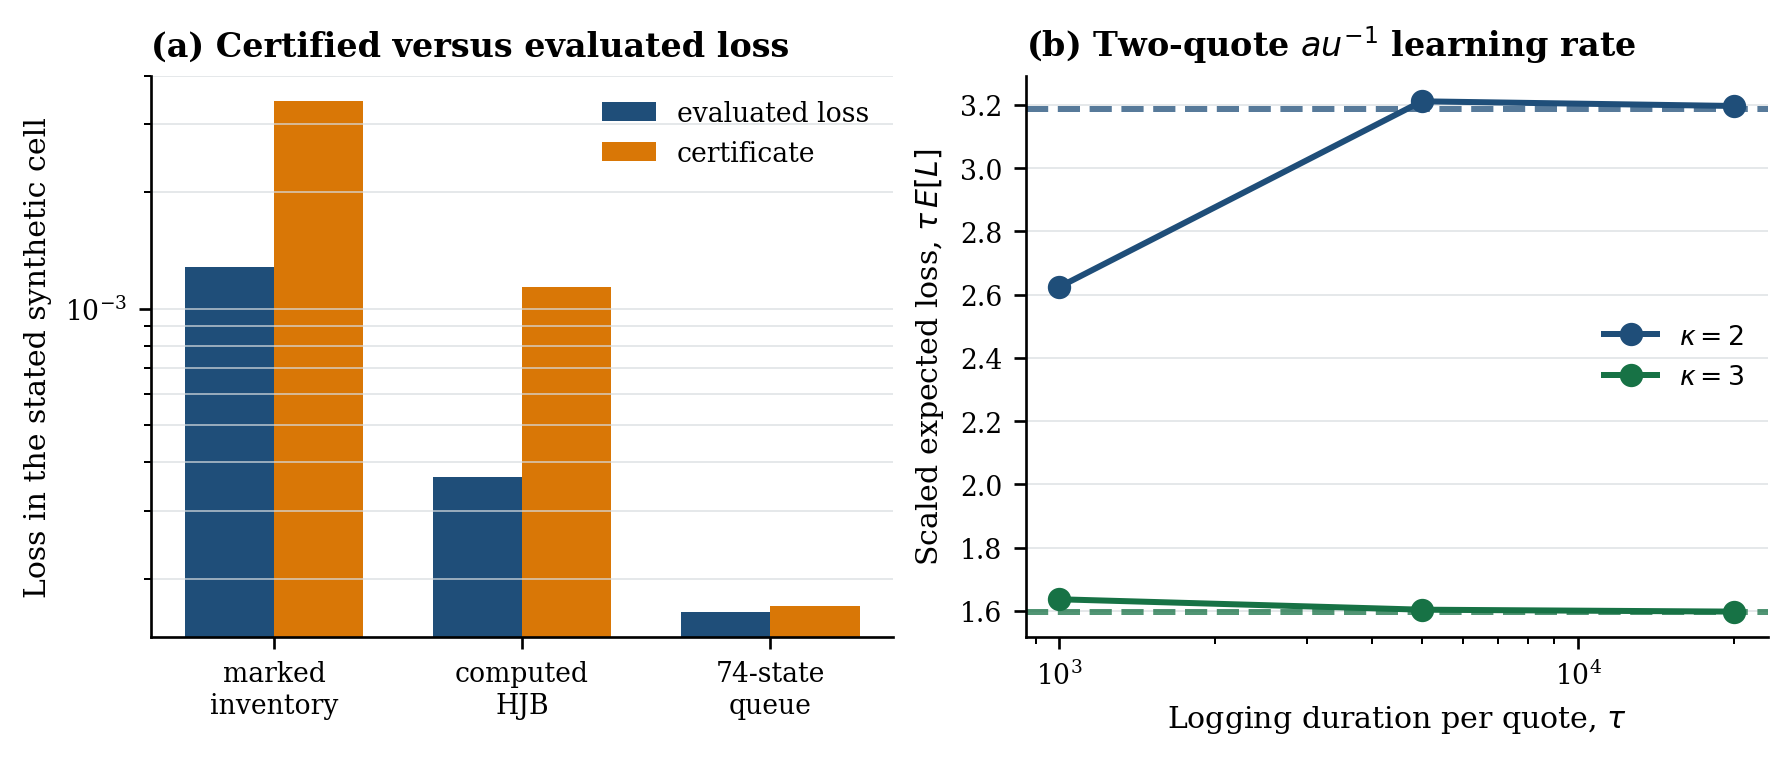
\includegraphics[width=\linewidth]{figures/05_certificates_learning.png}
\caption{Certificates and learning rates in separate synthetic cells.
Panel (a) compares independently evaluated policy loss with its applicable
certificate for the marked-inventory model, the computed HJB model, and the
74-state queue model; the logarithmic scale is shared, but each pair retains
its own declared model units. Panel (b) shows exact Poisson-sum evaluations
of \(\tau\E[L]\) for \(\kappa=2,3\), converging to the constants in
\eqref{eq:twoquoteasymptotic} (dashed lines). No simulated sampling or market
data are used.}
\label{fig:certificateslearning}
\end{figure}


\subsection{Partial fills during a pending cancel}
\label{sec:latencyexample}

Use the compound-consumption example of
Corollary~\ref{cor:compoundfills}, initially with three lots ahead
and a two-lot bid. Keep states \((n,m)\) with
\(n\in\{0,1,2,3\}\), \(m\in\{1,2\}\), and one fully filled
state \((0,0)\). Inventory is \(q=2-m\), so the live reservation
satisfies \(q+m=2\). These nine states describe the order during
one pending cancellation; no new orders are submitted.

Aggressive arrivals have rate \(1.4\), with batch sizes one and
three of probabilities \(0.7\) and \(0.3\).
The bid price remains fixed at \(99.98\). The marking reference
is \(S(2)=100\), \(S(1)=99.99\), and \(S(0)=99.84\), where its
argument is the remaining tagged quantity. These are declared
state valuations in this finite episode.
The offset before each event is therefore state dependent:
\(\delta_m=S(m)-99.98\).
Every consuming event uses its full wealth increment
\[
 g_e=f\delta_m+(q+f)\{S(m-f)-S(m)\}.
\]
This includes revaluation of shares filled earlier. A first
one-lot fill increases marked wealth by \(0.01\); a subsequent
fill of the remaining lot changes it by \(-0.29\). A two-lot
sweep directly from the initial inventory changes it by
\(-0.28\). The same final cash and marked inventory are obtained,
while discounting and running costs can distinguish the timing.
The generator thus retains the association between consumed
volume, executed quantity, and the complete price mark.
The running inventory cost is \(0.03q^2\),
the discount rate is \(\beta=0.8\), and the post-acknowledgement
value is the specified inventory penalty \(w=-0.05q^2\).
While acknowledgement is pending, that running cost continues
even if the order has already filled completely.

\begin{center}
\begin{tabular}{@{}rrrr@{}}
\toprule
Delay \(d\)&Probability of any fill&Expected filled lots&Pending value \(V^d\)\\
\midrule
0.01&0.00004958&0.00005858&\(-0.00000591\)\\
0.12&0.00655206&0.00808693&\(-0.00087478\)\\
0.35&0.04702895&0.06281535&\(-0.00722870\)\\
0.80&0.18180674&0.27252734&\(-0.03035474\)\\
\bottomrule
\end{tabular}
\end{center}
The probability of any fill and the expected filled volume are
different risk quantities. The table's marked value also includes
the dependence of fill quality on batch size and the inventory
remaining after cancellation. Instantaneous cancellation would
give zero value at the initial state.

Figure~\ref{fig:pendingcancel} traces these quantities over the complete
delay interval rather than only at the four tabulated delays.

\begin{figure}[tbp]
\centering
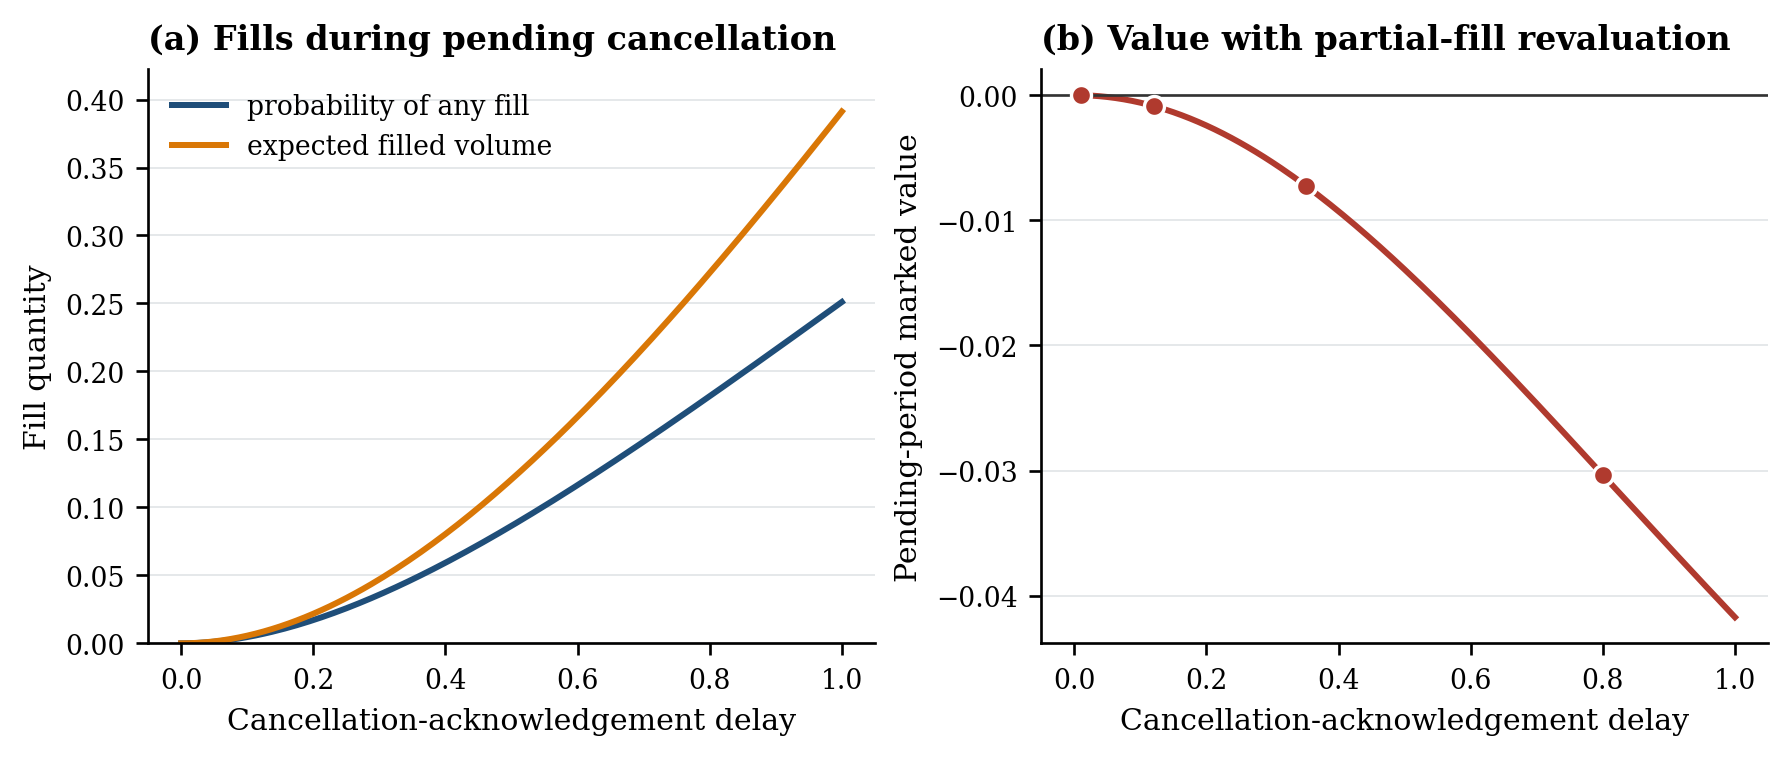
\includegraphics[width=\linewidth]{figures/03_pending_cancel.png}
\caption{A still-live order during cancellation latency. Starting with
three lots ahead and two tagged lots, panel (a) evaluates the compound
Poisson law for the probability of any fill and expected filled volume.
Panel (b) evaluates the exact pending-period value \(V^d\), including the
revaluation of earlier partial fills and post-acknowledgement inventory.
The markers are the four delays reported in the table. All quantities come
from the declared nine-state synthetic queue cell.}
\label{fig:pendingcancel}
\end{figure}

At \(d=0.35\), the residual constants of
Theorem~\ref{thm:erlanglatency} are exactly
\[
 G=\frac{303}{500},\qquad
 B=\frac{3473}{2500},\qquad C=\frac{38763}{12500}.
\]
The uniform expected-value approximation bound is
\(Bd^2/(2k)=0.08508850/k\).
\begin{center}
\begin{tabular}{@{}rrr@{}}
\toprule
Erlang stages \(k\)&Initial-state bias \(V^{D_k}-V^d\)
 &Uniform absolute bound\\
\midrule
4&\(-0.00112257\)&0.02127213\\
16&\(-0.00031387\)&0.00531804\\
64&\(-0.00008077\)&0.00132951\\
128&\(-0.00004058\)&0.00066476\\
\bottomrule
\end{tabular}
\end{center}
The scaled initial-state bias tends to \(-0.00521944\), the
coefficient \(d^2(e^{dA}Ag)_x/2\) in
\eqref{eq:erlangexpansion}. The uniform bound covers all nine
initial states and need not be attained at the displayed one.

Figure~\ref{fig:erlangapproximation} shows both the finite-stage error and
the sharp asymptotic normalization.

\begin{figure}[tbp]
\centering
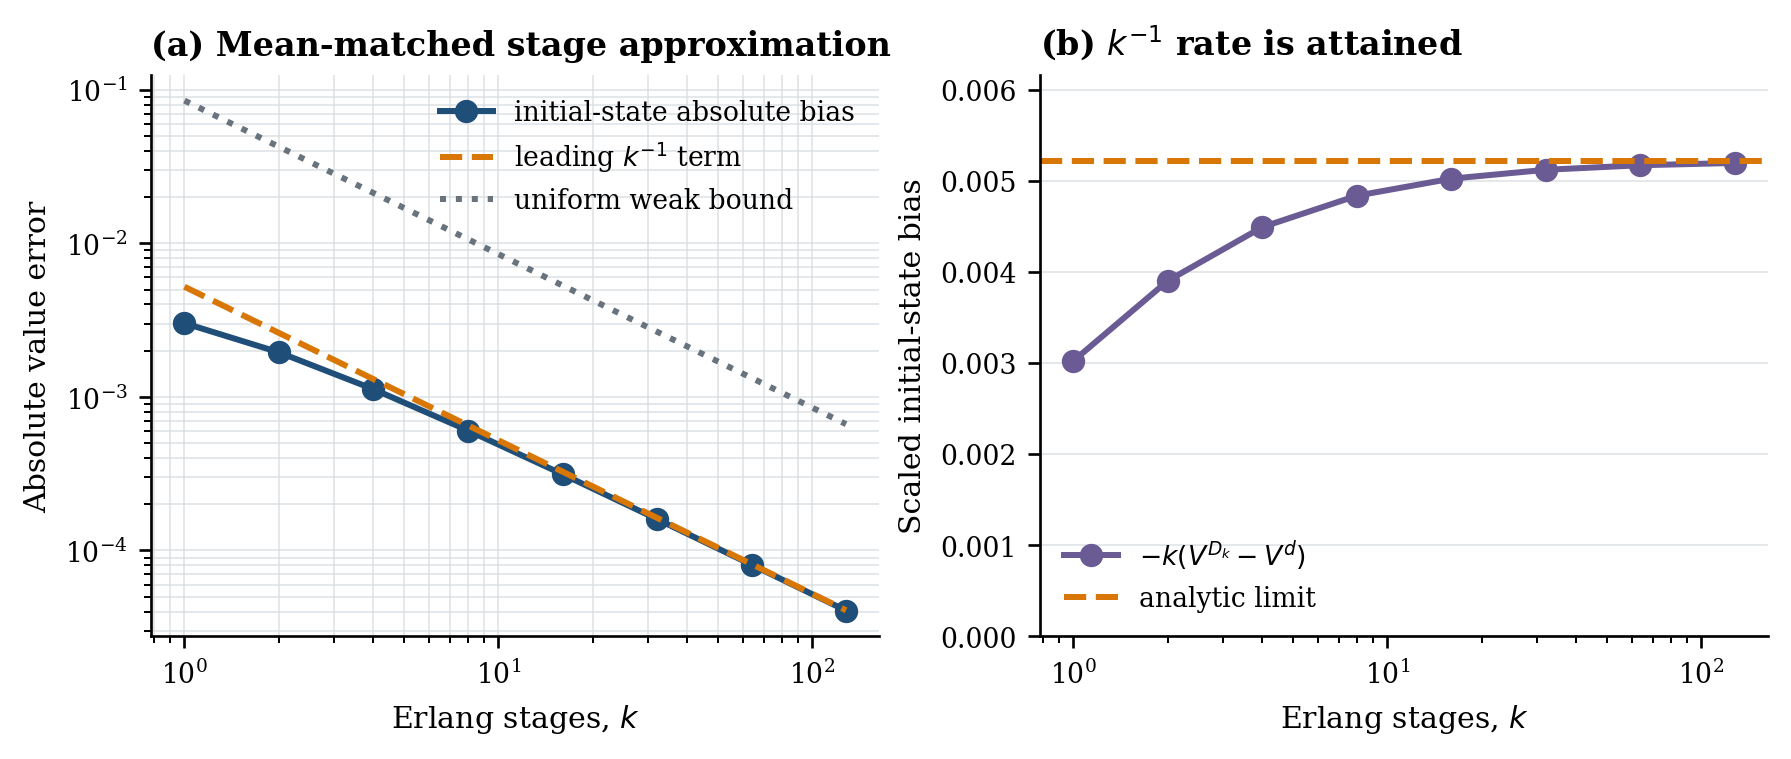
\includegraphics[width=\linewidth]{figures/04_erlang_approximation.png}
\caption{Mean-matched Erlang approximation of deterministic cancellation
latency at \(d=0.35\). Panel (a) compares the initial-state absolute bias
with the leading \(k^{-1}\) term and the uniform weak bound from
Theorem~\ref{thm:erlanglatency}. Panel (b) shows that
\(-k(V^{D_k}-V^d)\) approaches the analytic coefficient \(0.00521944\).
The independent stage recursion and matrix calculation use the same
nine-state synthetic cell as Figure~\ref{fig:pendingcancel}.}
\label{fig:erlangapproximation}
\end{figure}

The supplement compares the partial-fill distributions with direct
compound-Poisson sums in 32 cases and their generating functions
at 128 parameter points. Their largest distribution discrepancy
is below \(2\times10^{-15}\).
Matrix-exponential cancellation values agree with the residual
integral to below \(2\times10^{-16}\). Erlang stage recursions
are independently compared with matrix resolvents and integration
over the gamma density. The constants \(G,B,C\) use exact
rational arithmetic; the reported matrix values are floating-point
evaluations of the declared synthetic model.


\section{Scope and consequences}

The accounting identity applies to general admissible semimartingales.
The dynamic certificate uses a finite-state, translation-invariant model
and an additive marked-wealth objective. Its quadratic form requires a
common region with genuine curvature, whereas switching and tick choices
are covered by a uniform-error bound and, when supplied, an
occupation-margin refinement. The computable certificate also accounts
for HJB, terminal, and optimization errors. The shutdown threshold
concerns incremental gross markouts and does not override inventory
constraints or continuation values.

The event construction identifies the required queue and message
state, retains conditional fill marks, and maps event-law errors into
the control budgets. Replacement has a continuation-value cost because
it changes rank. A capped model also needs the separate exit allowance
in Proposition~\ref{prop:booktruncation}. These modeling terms remain
present even if its numerical HJB is solved exactly.
The interval message certificate accommodates discrete queue decisions
directly and retains their state occupation. Its numerical example
encloses an entire declared rate-and-reward box, with explicit
outward rounding. A model family that changes message maps or
the observation class requires an additional comparison.
Batch fills preserve the reservation pathwise but change both the
execution-volume law and the conditional mark contribution.
The cancellation-delay identity retains these fills until
acknowledgement. Its finite-stage approximation has an explicit,
sharp expected-value error bound under the stated independent-delay
law; dependence between congestion and future flow requires a
joint state model.

Three objects must be distinguished in calibration: the rate of fills,
the conditional law of their marks and destination states, and the value
function induced by those primitives. The certificate makes all three
channels visible, including the effect of an estimated value function.
The numerical supplement checks algebra and a synthetic finite-state
control problem, including a globally enclosed rational example.
Action coverage is a separate identification requirement: the
fixed-quote counterexample prevents vanishing statistical guarantees
from being inferred from sample size alone. The rank lower bound shows a distinct
information obstruction even when every primitive is known.
With rank observed, the replacement-boundary experiment has a
matching minimax rate of order \(\tau^{-1/2}\), whereas smooth
strongly curved choices can have quadratic estimation loss.
The two-quote construction
supplies a positive learning guarantee for a specified exponential cell,
including an unknown intensity scale. Discounting removes the terminal
horizon while retaining dependence on an effective horizon and the
curvature modulus. The signal-value extension replaces bounded losses
by a uniform centered moment condition. None of these results
supplies a fitted market model or a statistical confidence set without
the additional data and inference assumptions that such a set requires.

\bibliographystyle{plainnat}
\bibliography{references}
\end{document}
